%% main.tex -- "From Lagging to Leading: The Measured Emergence of Standing
%% Capacitance Behind Consumer Connections, 1997--2025"
%% (v5 identity per V5_RESTRUCTURE_SPEC_20260807.md: the measured identification
%%  of a new term -- trajectory -> decomposition -> load-independence ->
%%  connection scaling -> labelled EMC-filter hypothesis -> implications.)
%%
%% D. J. Hume, Electricity Authority (EA hat; descriptive, not policy advocacy).
%% Target venue of the condensed tier: IEEE Transactions on Power Systems
%% (TPWRS; re-pointed 17 Aug 2026 from OAJPE). This extended tier is the
%% complete record; it is not submitted, it accompanies the Zenodo package.
%%
%% Single source of truth for every number and figure: ../replication/ .
%% If a figure or number changes, change it in the replication notebooks first,
%% re-run, and it flows here (figures are pulled from ../replication/figures/).
%%
%% Build:  pdflatex main && bibtex main && pdflatex main && pdflatex main
%% (IEEEtran.cls and IEEEtran.bst are bundled in this directory.)

\documentclass[journal]{IEEEtran}

\usepackage{graphicx}
\usepackage{amsmath}
\usepackage{amssymb}
\usepackage{booktabs}
\usepackage{array}
\usepackage{url}
\usepackage[hyphens]{xurl}
\usepackage{orcidlink} % renders the ORCID iD icon; pulls in hyperref + tikz

% Figures live in the replication package (the single source of truth) and,
% as a fallback, in a local figures/ copy.
\graphicspath{{../replication/figures/}{figures/}}

\begin{document}

\title{From Lagging to Leading: The Measured\\
Emergence of Standing Capacitance Behind\\ Consumer Connections, 1997--2025}

\author{D.~J.~Hume~\orcidlink{0009-0006-6920-0598}%
\thanks{D. J. Hume is with the Electricity Authority, Wellington, New Zealand
(e-mail: corresponding author details on submission).
ORCID iD: \url{https://orcid.org/0009-0006-6920-0598}.}%
\thanks{This is descriptive analysis of public regulatory metering and
information-disclosure data. The views expressed are the author's. No external
funding was received. The analysis informs, but does not advocate, a live
reactive-power pricing policy question (Section~VI-D).}%
\thanks{A reproducibility package (the analysis notebooks that compute every
number and figure in this paper from public data) accompanies the work.}%
\thanks{This is the \emph{extended version}, including the complete
measurement-error analysis (Appendix~A), the mains-filter appendix, and
supporting exhibits; a condensed version is prepared for submission to the
IEEE Transactions on Power Systems.}}

\markboth{Extended version --- a condensed version is prepared for submission to the IEEE Transactions on Power Systems}%
{Hume: The Measured Emergence of Standing Capacitance Behind Consumer Connections}

\maketitle

\begin{abstract}
Both ENTSO-E Final Reports on the 2025 Iberian and North Macedonian blackouts read the excess capacitive reactive power as a network term---the reading the available data supports. The Iberian report asks for what was missing: information on load composition. We build that record from regulatory half-hourly metering at New Zealand's transmission--distribution
boundary, spanning 29 years, and find a second source: the demand behind the
customer's connection, at mains voltage and in residential, commercial and
industrial premises alike, has itself moved capacitive. Overnight reactive
power crossed from lagging to leading in 2016, nearly a decade before the 2025
events, and a first-principles charging calculation puts the demand-side share
of that drift in the physical band 75--88\%. That term behaves as a net standing shunt
element---present around the clock, scaling with the connections served, and
moving capacitive by about 210~VAr per connection over 2013--2025 and roughly
20~VAr a year at the close. It drives the drift rather than the level: the
distribution network's own cable and line charging remains the larger part of
the standing leading reactive power, and what changed is that a demand once
strongly lagging stopped masking it. The candidate device layer is the
electromagnetic-compatibility filter mandated in nearly every mains-connected
product (a labelled hypothesis): a few VAr per device, tens of devices per
household, millions across a system and perhaps billions on the
largest---permanently across the mains and switched by nobody. Its injection
rises with the square of mains voltage, so every 230-volt system accumulates about three times more per device than a 120-volt, 60-hertz one. Planning and protection studies still carry a constant
lagging load archetype, where the overnight flow now has the opposite sign.
Both inputs to the measurement are records any operator already holds.
\end{abstract}

\begin{IEEEkeywords}
Reactive power, power factor, overvoltage, leading power factor, shunt
capacitance, distribution cabling, measurement, grid exit point, load
composition, load modelling, power-system analysis.
\end{IEEEkeywords}

% ======================================================================
\section{Introduction}
% ======================================================================
\IEEEPARstart{P}{ower} systems internationally are shifting from net-absorbing
(lagging) toward net-generating (leading) reactive power at light load, as the
connected load fleet modernises toward power-electronic devices and networks add
underground cabling. The direction of the transition is not in dispute, and
this paper does not claim to be the first to observe it. What has been missing is,
first, a long \emph{measured} record of the transition observed end to end at
supply-point resolution, and second, a measured separation of how much of the
drift is the load fleet and how much is the network. This paper supplies both for
a single national system, connects the result to a failure mode that has
recently moved from theory to realised blackouts, and closes with what the
reversal implies for the analysis and defences that were built for the opposite
regime. The trail leads somewhere unexpected: to the electromagnetic-compatibility
filter inside every mains-connected device---capacitance that one part of the
regulatory apparatus requires and no other part counts---advanced here as a
labelled hypothesis with its decisive test identified.

\subsection{A global reactive transition, already observed}
The phenomenon is well attested across jurisdictions. In Great Britain, Kaloudas
\emph{et al.}~\cite{kaloudas2014,kaloudas2017} documented a steep decline in
reactive demand at minimum load, with distribution networks beginning to export
reactive power to the transmission system; in France, the transmission operator
attributes off-peak overvoltage episodes to a three-factor mechanism of
distributed generation, underground cabling, and evolving final
consumption~\cite{rte_bilan}; in Australia, Powerlink Queensland links a rising
likelihood of overvoltage events partly to more energy-efficient appliances
alongside rooftop solar~\cite{powerlink_seq}. Rising capacitive export to the
extra-high-voltage network has likewise been reported in continental
Europe~\cite{tazky2021}. At device level, Hannagan \emph{et
al.}~\cite{hannagan2023} found the majority of modern household appliances
present a leading power factor, and international expert reviews reach
consistent conclusions about modern lighting and power electronics and about
the error introduced by constant-power-factor load
modelling~\cite{cigre_tb719,epri_loadmodel}. No consumer-device standard requires
a unity fundamental-frequency (displacement) power factor: IEC~61000-3-2 limits
harmonic current only~\cite{iec61000_3_2}, and a 2020 amendment removed the
last power-factor term from its limits. The one device-level power-factor
family in force anywhere---the European, and from 2026 Australian, lighting
floors~\cite{eu_lighting2020}---is a full-load, direction-blind metric that
never sees a device's standing draw, and it has no New Zealand counterpart.
The European Demand Connection Code remains the only international instrument
addressing reactive exchange at the demand connection
point~\cite{eu_dcc}. The
overvoltage-instability literature itself now records the observable: the 2026
review of overvoltage instability mechanisms notes, among its causes of voltage
rise, that cable substitution has ``change[d] the power factor to leading in
several urban substations''~\cite{vournas2026review}---an observation offered
without citation, and attributed wholly to the network's cables rather than to
any change in what the connected demand draws. Every system in this literature
runs 230-volt mains; Section~V-B returns to that regularity.

\subsection{Prior measurement and decomposition}
The closest measured system-level series is the British one~\cite{kaloudas2014,
kaloudas2017}, which characterises roughly eight years (about 2005--2013) of
reactive demand at grid supply points and projects the trend forward from
load-composition modelling and scenario projection; it supplies neither a
multi-decade measured record nor a quantified demand-versus-network share of
the realised drift. At the transmission--distribution interface, Javed
\emph{et al.}~\cite{javed2024} characterise the consequences of capacitive
reactive export in a Netherlands network, Baghban-Novin \emph{et
al.}~\cite{baghbannovin2020} simulate feeder undergrounding and distributed
generation on a Danish test system, and a Slovak study~\cite{tazky2021} links
growing capacitive flow into the transmission network to the changing nature
of the distribution network; none is a long measured record and none
attributes a quantified demand-versus-network share.

The single study closest to the present decomposition is Bosisio \emph{et
al.}~\cite{bosisio2022} on the Milan distribution network. Using measured
15-minute active and reactive power at 37 high-voltage/medium-voltage
transformers, it names the same three-term balance at the
distribution--transmission boundary used here---the reactive power withdrawn or
injected by customers, that consumed by the cables' inductance, and that
produced by the cables' capacitance---and in the indexed English-language
literature it is, to our knowledge, the only prior study to articulate this
split explicitly on measured boundary data. It differs from the present work
on three points that matter: it compares two years (2019 against 2020, across
a COVID-19 demand shock) rather than a multi-decade drift; it assigns no
numerical share to the three terms; and where it attributes dominance it
concludes that the leading flow follows from the capacitive nature of the
Milan cables, with reduced demand amplifying rather than causing it---on which
term dominates, its reading runs opposite to ours. We treat it as
complementary: it confirms the framework on measured data for one heavily
cabled city, its cable-dominant reading for that network is consistent with
our own cohort result that cable intensity shapes where net-leading territory
is reached first (Section~IV-A), and it leaves open the national,
multi-decade, quantified attribution.

\subsection{The realised risk}
In 2025 two power systems suffered major blackouts whose official investigations
found a leading-reactive/overvoltage mechanism at their core: the Final Reports
of the European Network of Transmission System Operators for Electricity
(ENTSO-E), both published 2026, on the Iberian Peninsula event of 28 April
2025~\cite{entsoe_iberia} and on the North Macedonia event of 18 May
2025~\cite{entsoe_nm}, detailed in Section~VI-C. What matters here is what those
investigations could not do. Both reports treat the capacitive surplus as a
network-side quantity and low demand as a magnitude rather than
as a fleet whose reactive character has itself changed; neither distinguishes nor
quantifies a demand-side composition shift from network charging. The Iberian expert panel models the reactive response of load to voltage, but its load model's
reactive voltage exponents come from a table of typical values by load
class---how the reactive power of demand varies with voltage, not what it
was---and the North Macedonian report carries no load power-factor assumption
at all; on two independent full-text reads of each report, neither states the
aggregate reactive character of demand anywhere. The Iberian panel names the gap itself: modelling the transmission--distribution interfaces accurately, it notes, would need ``information on load composition''~\cite{entsoe_iberia}. These are not criticisms of
investigations that reasoned from the data available to them; they identify the
space a long measured record can fill. The field's current synthesis has the
same shape: the 2026 mechanisms review~\cite{vournas2026review} gives as its
causes of voltage rise corridors below surge-impedance loading, cable
substitution, synchronous-generator decommissioning, and fixed-power-factor
converter operation---network and generation throughout---representing load as
lagging or unity power factor in every model, citing no measurement of demand
reactive character, and calling for none.

Operational practice has the same shape. Australia's transmission connection
point forecasting methodology computes power factor at the
transmission--distribution boundary from measured active and reactive power, and
labels each point leading or lagging; but it takes that reading from the top
1\% of half-hours ranked by active power, and holds the power factor constant
over the forecast horizon~\cite{aemo_tcpf}. Where it does anticipate the
light-load power factor changing, it attributes the change to inverter
standards. The measurement is made, at the peak.

\subsection{Contribution}
This paper makes a layered contribution.

\emph{Contribution~1 (measured trajectory).} Using regulatory half-hourly active
and reactive power at New Zealand grid exit points, we measure the system's
reactive character at supply-point resolution over 29 years (1997--2025) on a
balanced panel---the same grid exit points in every year, so sites entering or
leaving the record cannot manufacture the trend---characterise its rate and
crossing, and show the trajectory is a measured phenomenon and not a metering
artefact. The computation
reuses settlement metering that any operator holds, so the same measurement is
available to any system.

\emph{Contribution~2 (decomposition of the drift).} We decompose the drift into
a demand-side load-composition component and a distribution network cable-charging component. The magnitude is carried by a first-principles charging calculation
that computes each network's cable charging directly from its disclosed
circuit kilometres (Section~II-D) and so fits no cable coefficient; evaluated
over the 2013--2025 disclosure window, it puts the demand-side (\emph{organic})
share of the drift at about 80\% (physical band 75--88\%), with two statistical
methods corroborating the direction over the full 29-year record but not
themselves pinning the share. We report a measured direction and dominance and
do not claim a point-identified split.

\emph{Contribution~3 (the term identified).} We then identify what the
demand-side driver is physically doing. The deepening is load-independent---as
large at the flat evening peak as overnight---so it behaves as a standing shunt
element, permanently energised, not as a change in how the load draws
reactive power while operating. And it lives behind the connections: across
grid exit points the 2013--2025 deepening is proportional to the number of
connections served, with no detectable connection-independent residual; refitted
year by
year, each connection's standing contribution sits slightly on the inductive
side of zero at the start of the record, crosses zero early in the 2010s, and
grows every
year thereafter---about 210~VAr per connection added over 2013--2025, read off the
level history and reproduced within 10\% by the fitted endpoint
change---and it accumulated faster over the second half of that window than
the first
(Section~V). The load fleet's own standing shunt term is moving capacitive,
not merely drawing fewer lagging vars. We advance the mandated
electromagnetic-compatibility filter capacitance as its candidate device layer
(a labelled hypothesis), identify the decisive low-voltage measurement that
would settle it, and note that both of the scaling test's inputs---settlement metering
and connection counts---are records any operator holds.

The significance is what the reversal does to analysis: the direction of the
binding voltage-security question reverses; the automatic last-resort defences
and the margin tooling of the undervoltage era do not transfer; and the
constant-lagging-power-factor load archetypes of planning and protection
studies no longer describe the light-load fleet (Section~VII)---a qualitative
synthesis, not a defence-scheme or load-model redesign, which remain outside
the paper's scope. Section~III measures the trajectory; Section~IV attributes
it between fleet and network; Section~V identifies the term and tests its
scaling; Sections~VI and VII set out the overvoltage consequences and the
analysis implications; Section~VIII collects future work.

This work extends the author's EEA~2025 conference paper~\cite{hume2025}, which
described the 2009--2024 aggregate trend qualitatively. The present paper adds
twelve further years of baseline back to 1997, in the firmly lagging regime;
grid-exit-point spatial resolution; a quantified rate and crossing with an
explicit artefact test; the decomposition of the drift; the connection-scaling
identification; and the two post-EEA ENTSO-E Final Reports as an independent
evidentiary anchor. Consistent with its descriptive scope, the paper reports the
measured trajectory and the decomposition and notes that they inform a live
reactive-power pricing question, without making any policy recommendation.

% ======================================================================
\section{Data and Method}
% ======================================================================
\subsection{Sign convention and primary variable}
Reactive power carries a direction that is the entire point of this study. We use
the convention $Q<0$ for \emph{leading} (capacitive, voltage-raising) and $Q>0$
for \emph{lagging} (inductive, voltage-lowering). We lead throughout with the
signed reactive power in MVAr, which is additive across supply points and has no
discontinuity at unity, and present power factor only as a familiar comparator.
Power factor is non-additive, so where a system power factor is quoted we sum $P$
and $Q$ across the panel first and derive
$\mathrm{PF}=\Sigma P/\sqrt{(\Sigma P)^2+(\Sigma Q)^2}$ rather than averaging
power factors.

\subsection{The grid-metering record and the balanced panel}
The primary data is half-hourly real and reactive power at every grid exit point
(GXP), the substations where the national transmission grid hands electricity to
the local distribution networks, from 1997 to 2025, published by the New Zealand
Electricity Authority on its Electricity Market Information (EMI) platform. Each per-year
file is half-hourly for the whole year, indexed by trading date and trading
period (48 half-hour periods per day), with a real-power and a reactive-power
column for each GXP. Over the record, 238 distinct GXPs appear; a balanced core of
132 is present in all 29 years.

The series exists because a rule required it. The Electricity Governance Rules
obliged the Electricity Commission to establish and maintain a centralised data
set to support planning~\cite{egr_partf_r11}, and the half-hourly record
assembled for it in 2004 was drawn from the settlement metering of the market's
own start, running back to 1~October 1996---the old metering files of the
Electricity Corporation of New Zealand, the state enterprise that once owned
both generation and the grid, and the MV90 and Avalon systems that succeeded
them~\cite{ec_cds2004}. Its stated reason for inclusion was demand forecasting
and the Grid Investment Test: active-power problems. Reactive power entered that
specification only as a plant parameter---generator reactive ranges, station
voltage control, capacitor bank kVAr. The reactive column at the boundary has
therefore been recorded for twenty-nine years because settlement metering
records it, not because it was the object of anyone's question.

We reduce each GXP's year to a small set of features, of which the headline
quantities are the average overnight and evening-peak reactive and real power.
Following the prior EEA analysis, the overnight window is trading periods 6--10
(approximately 02:30--05:00, the deepest part of the night and the lowest demand)
and the evening peak is trading periods 36--38 (approximately 17:30--19:00). We
also record, for each GXP-year, the fraction of overnight half-hours that were
leading. The full feature table is 5{,}261 GXP-year rows, one per GXP per year.

The single largest way a 29-year trend could be spurious is a change in the set of
measured GXPs over time: new urban, cable-heavy sites appearing and old rural ones
dropping out would manufacture a leading trend from bookkeeping alone. The primary
defence is the \emph{balanced panel}: only the 132 GXPs present in every one of the
29 years, so any change is a change in the same sites rather than a change in which
sites are measured. We call that turnover---grid exit points entering and leaving
the measured set---\emph{churn}; the balanced panel is churn-controlled by
construction (``balanced'' in the panel-data sense, the same sites in every year,
not the three-phase sense). We follow one rule throughout: \emph{trends on the balanced
panel, snapshots on the full panel}. The paper's subject is the distribution
networks; restricting the balanced panel to demand networks (excluding a handful of
generator, industrial, and rail connection points) leaves 123 GXPs. We report both
the 132-point and 123-point figures and keep them labelled; they are the same trend
at the same rate (Section~III). The residual churn bias is signed: the demand grid
exit points excluded from the balanced panel (post-1997 entrants and exits) are by
2025 on average \emph{more} leading than the panel (median $-0.28$ against
$-0.18$~MVAr/MW) and drift faster ($-0.020$ against $-0.018$~MVAr/MW/yr), so the
balanced panel, if anything, understates the national drift.

\subsection{Metering provenance and accuracy}
The active and reactive power at each grid exit point is settlement-grade revenue
metering owned by the national grid owner and system operator (Transpower), the
registered metering equipment provider for these points. Grid metering is the
highest-accuracy category of the regulatory Metering Code~\cite{eipc_part10},
certified by an approved test house and periodically re-certified and inspected. The
present fleet is Schneider PowerLogic ION8800A meters, Class~0.2S for active energy
under IEC~62053-22~\cite{iec62053_22}, four-quadrant (import and export active and
reactive), with Class~A power-quality measurement under
IEC~61000-4-30~\cite{iec61000_4_30}, installed across roughly 150 grid sites in
2010--2013~\cite{transpower_amp}, replacing legacy PSI~Quad4 meters dating from
about 1994~\cite{transpower_amp2010}; the reactive series thus rests on four-quadrant
revenue metering for the modern record and on the older, coarser Quad4
instrumentation for the early record.

At a grid exit point the active-energy channel is held to Class~0.2 while the
reactive channel is held to the looser Class~2--3 (about $\pm 2$--$3.5\%$) of
IEC~62053-23~\cite{iec62053_23}, with reactive accuracy specified only above 20\% of
rated current; as a share of the reading, reactive measurement is least
accurate at light load and near-unity power factor, where the reactive component is
small while current-transformer phase-angle error is largest. This asymmetry is the
international norm, because active energy is the settled quantity. The reactive
energy of the metering standards is the fundamental-frequency
(\emph{displacement}) quantity of IEEE Std~1459~\cite{ieee1459}: the reactive
power set by the phase angle between the voltage and the 50-Hz component of the
current. The harmonic currents
drawn by power-electronic loads add apparent power (distortion power) but
accumulate no reactive energy on the meter, so the trend measured here is in
fundamental-frequency reactive power---the component that drives the voltage rise
of Section~VI---with harmonic distortion out of scope. The cited standard does
not by itself settle which quantity a given meter records, and the standards are
moving on the point: the classes of IEC~62053-23 are being withdrawn into
IEC~62053-24. The record supplies the check the standard does not. A distortion
component would scale with the load operating, and so would concentrate in the
loaded evening window---where Section~V-A measures the deepening as near-equal
in both, the same structure that bounds the $P\sin\beta$ term.

Neither the accuracy classes nor the one metering transition in the record can
account for the measured drift; Appendix~A carries the arguments in full.
Class-bounded \emph{random} error is bidirectional, averages down under
aggregation, and cannot manufacture a near-monotonic 900-MVAr swing through
zero; the one error that does \emph{not} average down (a systematic
current-transformer phase-angle bias of the form $P\sin\beta$, concentrated in
exactly the light-load window this paper measures) is bounded in Appendix~A to
a near-static offset some fifty times smaller than the swing, contributing
about 0.1~MVAr/yr of apparent drift; the staggered 2010--2013 fleet
replacement is anchored out by the record's endpoints, with the modern-era
drift, if anything, steeper; and a test for a synchronous system-wide re-base
finds none. We therefore treat the multi-decade \emph{drift} as robust while
regarding the standing reactive \emph{level} on any single night as carrying
more measurement uncertainty, consistent with the level being the weaker claim
of Section~IV.

\subsection{The asset (parameter) record}
To describe each network's physical make-up we assemble a per-company, per-year
table from the Commerce Commission's regulated information disclosures: circuit
length split into overhead and underground kilometres at each operating voltage
(Schedule~9c, disclosed consistently from 2013), capacitor-bank counts
(Schedule~9a), demand and connection counts
and embedded generation (Schedule~9e), and the regulated asset base (Schedule~4).
The disclosures are mapped to the EMI network codes through a 29-year validated
correspondence, time-aware because ownership itself changed under the record: 34
demand grid exit points (32 of them in the balanced panel) changed network code,
almost all from the breakup of UnitedNetworks and the onward sale of its
Wellington network (successor codes appear 2003--2013), plus one Nelson-region
boundary change. The metering panel is attributed per year from the metering
files themselves, so the trajectory follows every change; the cable-dose
analyses of Section~IV are run under both a per-year and a physical-continuity
(successor-network) attribution, with the sensitivity reported there. Two data-quality choices are made explicitly: we retain only the
``All''-network roll-up rows so that multi-network companies are not double
counted, and we flag a 2014--2015 definitional break in the capacitor counts (a
widening of reporting scope, not new plant) so that a paperwork change is never
read as a physical one. The capacitor series is counts only, with no MVAr ratings
or installation dates, and begins in 2013; we use it as a direction-only
proxy---a stand-in that can indicate direction, not size.

\subsection{Confounds in the metered reactive power}
A grid exit point meter records the \emph{net} reactive power at the boundary, which
is not in general a clean distribution offtake:
\begin{equation*}
Q_{\text{metered}} = \underbrace{Q_{\text{load}} + Q_{\text{cable}}}_{\text{the subject of this paper}}
\;-\; Q_{\text{embedded gen}} \;\pm\; Q_{\text{TP plant}},
\end{equation*}
where the last two terms are \emph{confounds}: signals mixed into the same
metered reading that are not the subject of this paper. An embedded \emph{synchronous} generator
(hydro, geothermal, or cogeneration) regulates voltage and sets its reactive output
by the voltage it sees rather than by local load; and at some substations a
Transpower voltage-regulating device (a static var compensator or static
synchronous compensator (STATCOM), a
synchronous condenser, or a switched capacitor or reactor bank) shares the
substation with the offtake, with the revenue-metering boundary determining
whether it registers in the metered flow. One behavioural diagnostic catches all of these,
whichever party owns the plant---a network's own large regulating compensation
would be flagged identically: a clean distribution offtake's reactive power tracks
its load, so a straight-line fit predicting $Q$ from $P$ explains an appreciable
share of its variation ($R^2 \approx 0.3$--$0.5$), whereas voltage-regulated
reactive is decoupled from load ($R^2 \to 0$, with a large residual the load
does not explain). Computed on three
spread-out years (2016, 2019, 2022) so that a flag reflects a stable trait, the screen isolates six \emph{decoupled} grid exit
points---\emph{contaminated}, in the sense that the metered reactive power
includes plant that is not the distribution offtake, whether embedded generation
or transmission-owned voltage-regulating plant: ISL0661 and BRY0661 (Islington and
Bromley, Christchurch: substations hosting Transpower voltage-regulating
plant---static var compensators, switched capacitor banks, and shunt
reactors---and serving a distribution network extensively reconfigured after
the 2010--11 earthquakes), PEN1101 and HOB1101 (Auckland), BPE0331 (Bunnythorpe), and TWH0331 (Tuai,
with the Waikaremoana hydro stations).

This matters overnight specifically: the overnight minimum removes generation
that merely stops, but not plant that regulates voltage around the clock. That
includes the synchronous fleet---hydro, geothermal and cogeneration regulate
voltage whatever the hour---and, increasingly, inverter-based plant running a
night-time reactive mode, which holds a voltage setpoint at zero active power
and so is not removed by darkness either. The diagnostic above is behavioural
rather than technology-specific, so it catches both. One
illustrative public case is the Cobb hydro station, divested by Transpower to
Network Tasman around 2011: its pricing node was retired and its output now nets
into the Stoke grid exit point (STK0661), a ``lost node'' whose metered reactive no
longer represents a clean offtake. We flag these sites rather than discard them
silently, and we show in Sections~III-B and IV that the trajectory and the
decomposition are robust to their removal: the contamination affects the absolute
\emph{level}, not the direction, intensity, or attribution of the drift.

\subsection{Analysis methods}
The trajectory is summarised by ordinary linear slopes for headline rates and, for
robustness, by Theil--Sen slopes~\cite{sen1968}: the median of the slopes through
every pair of years (406 pairs for a 29-year series), an estimator that a few
anomalous years cannot move, standard in long-record environmental trend
monitoring, used here on both the national and per-GXP series; where the two
estimators agree---as they do throughout---a trend rests on no small set of
years. The test that the trend is not a metering artefact
(Section~III-B and Appendix~A) removes each GXP's own Theil--Sen trend and looks in what remains for a step
shared across sites in the same year, using a change-point detector and a
coherence statistic. The decomposition (Section~IV) uses three methods: a
clean-cohort comparison and a mixed-model cable dose-response with a
company-cluster bootstrap (validated on synthetic data before use), which share a common
underground-cable proxy and so are not independent of one another; and a
first-principles cable-charging calculation, $Q=\omega C V^2 \ell$, with a $\pm
35\%$ physical band on cable capacitance carried through to the result, which fits
no cable coefficient and is independent of the other two. All analysis is
reproduced from public data in the accompanying notebooks.

% ======================================================================
\section{The 29-Year Reactive Trajectory}
% ======================================================================
\subsection{Lagging to leading, overnight}
Fig.~\ref{fig:traj} shows the central empirical result. Summed across the balanced
demand panel, mean overnight reactive power fell from $+466$~MVAr (lagging) in 1997
to $-451$~MVAr (leading) in 2025, a near-monotonic linear drift of $-31.1$~MVAr/yr
(robust Theil--Sen slope $-31.3$~MVAr/yr, 95\% confidence interval (CI)
$[-34.0,-28.1]$, the rank-based interval taken as order statistics of the
sorted pairwise slopes~\cite{sen1968}, which like the estimator itself treats the annual values as
serially independent; since consecutive years are in fact strongly correlated,
read it as the spread among the pairwise slopes rather than a coverage
guarantee), crossing into
net-leading overnight in 2016. On the wider 132-point balanced panel
that also includes non-distribution connection points, the same drift is
$+673\rightarrow-296$~MVAr at $-30.3$~MVAr/yr, crossing in 2020; the rate is
essentially identical and the leading endpoint is, if anything, stronger on the
demand-only panel once lagging industrial load is removed. The two panels are the
same trend, labelled distinctly and never blended into one figure. Expressed per
megawatt of overnight load, the drift is about $-0.018$~MVAr/MW/yr; we lead with
this intensity and with the share of networks gone leading because, unlike the
absolute MVAr total, they are insensitive to a few large contaminated nodes
(Section~III-B). The denominator is not doing the work: overnight load on the
panel grew from about 1{,}680~MW in 1997 to about 1{,}960~MW in 2025. In the
familiar comparator of Section~II-A, the overnight aggregate power factor moved
from 0.964 lagging to 0.975 leading---a numerically small excursion either side of
unity concealing a 900-MVAr reversal, which is why the signed reactive power is
the working variable throughout.

\begin{figure*}[!t]
\centering
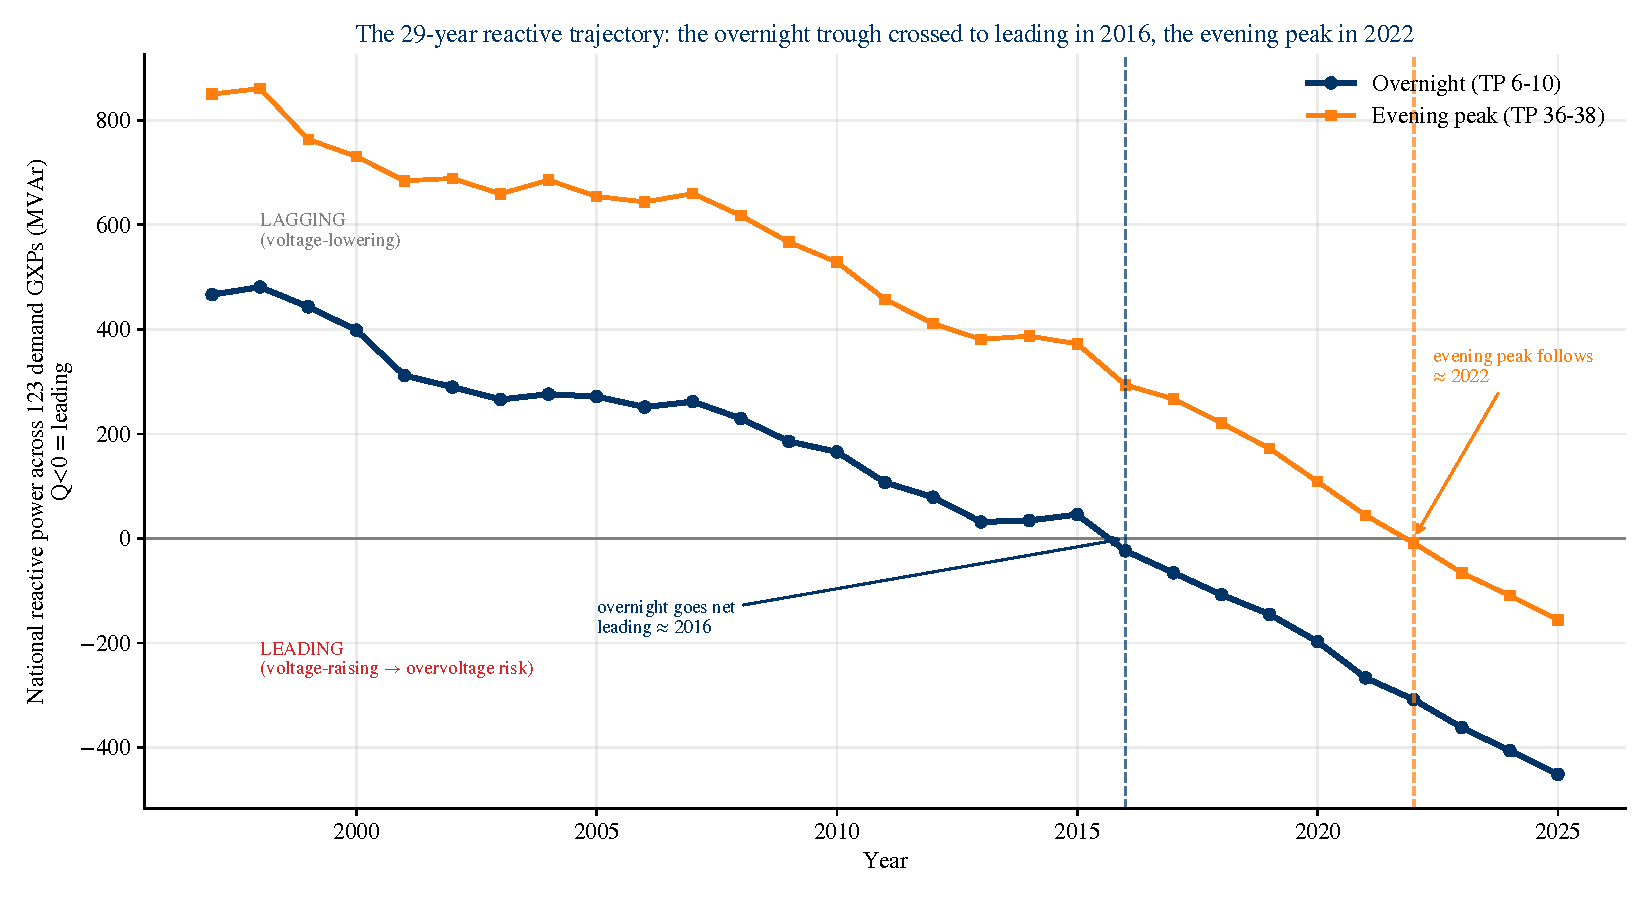
\includegraphics[width=0.74\textwidth]{01_trajectory.pdf}
\caption{The 29-year reactive trajectory on the balanced demand panel (123 grid
exit points present in all years). Overnight (trading periods 6--10) drifts from
strongly lagging ($Q>0$, voltage-lowering) to clearly leading ($Q<0$,
voltage-raising), crossing net-leading in 2016; the evening peak (trading periods
36--38) follows much later. The diurnal split (the problem lives overnight at low
load, not at the busy evening peak) is the signature of a standing capacitive
term dominating when load is least able to mask it; Section~IV attributes that
term mainly to the demand fleet rather than to network charging. Sign convention: $Q<0$ is leading.}
\label{fig:traj}
\end{figure*}

The diurnal contrast is itself a result. The evening peak crossed net-leading only
in 2022 and remains far less leading than overnight, which locates the net-leading
regime firmly at low load. Expressed as a
fraction rather than a sum, the mean share of overnight half-hours that are leading
rose from about 1\% in 1997 to about 74\% in 2025: overnight leading became routine
rather than exceptional.

\subsection{Measured, not an artefact; robust to contaminated sites}
Two features of the record answer the metering-artefact objection
directly, and a further test closes the one gap they leave.

First, the drift does not rest on the older, less homogeneous early data. The metering
and data pipeline modernised across the record (notably the move to the present
Electricity Market Information system), and the one visibly suspect feature is an early
step in the overnight leading fraction between 2000 and 2001, consistent with a change
in metering vintage. Restricting to the homogeneous modern era removes any such concern,
and the drift is if anything slightly steeper: $-33.0$~MVAr/yr over 2002--2025 against
$-31.1$~MVAr/yr over the full record. A trend manufactured by early-era inhomogeneity
would fade on the clean modern data, not strengthen.

Second, a measurement artefact cannot reproduce the trend's physical structure. The
net-leading crossing is specific to the overnight window---the evening peak stays
lagging for years longer (Fig.~\ref{fig:traj})---while the deepening beneath the
crossings is near-equal in the two windows over 2013--2025, with evening-peak load
essentially flat (Section~V-A): the signature of a standing capacitive term netted
against different amounts of lagging load. The one systematic metering bias that does
not average down scales with the metered load ($P\sin\beta$, bounded in Appendix~A)
and would deepen the heavily loaded evening window far more than the lightly loaded
overnight one, which is not observed. Nor is the shift seasonal: recomputed
separately for winter (June--August) and summer (December--February) months, the
overnight aggregate drifts at $-31.1$ and $-30.8$~MVAr/yr respectively, so the trend
is not an artefact of heating-season load composition. The drift also tracks each network's
underground-cable intensity (Section~IV); a metering error has no reason to
correlate with cable kilometres. Nor does a metering artefact at the grid
exit point have a mechanism that scales with the customers behind it: the 2013--2025 deepening grows
linearly with each grid exit point's connection count, and that
connection-scaling term carries the large majority of it (Section~V-C). This
combination of a diurnally structured, cable-correlated, connection-scaling
shift is one that a change in measurement convention cannot counterfeit. The
charging calculation of Section~IV is not a further witness here: it
\emph{partitions} the measured drift rather than reproducing it, so an
instrument error would sit inside the residual it assigns to the fleet.

These two arguments address a gradual or staggered change, such as piecemeal
meter replacement across sites. A single system-wide re-base---a one-date change
of sign convention or central processing that would step every supply point at
once---is different; we test for exactly that in Appendix~A and find no such
event. The lagging-to-leading drift is therefore a measured property of the
system, not an artefact of how it was metered.

A second objection, distinct from a metering artefact, is that the trend could be
carried by a few grid exit points whose meters do not see a clean distribution offtake
(Section~II-E). We test it directly by removing them. Dropping the six \emph{decoupled}
grid exit points whose reactive power is set by plant or embedded generation (the
\emph{clean} cohort), and more strictly also the steady-generation and net-export
points (the \emph{clean-strict} cohort), we re-measure the trajectory on the balanced
demand panel (Fig.~\ref{fig:clean}).

Two quantities behave very differently, and the difference is the point. The absolute
total and the MVAr/yr slope \emph{shrink} when the contaminated sites are removed---the
2025 total from $-451$ to about $-300$~MVAr and the slope from $-31.1$ to
$-23.4$~MVAr/yr---because two of the removed nodes (Islington and Bromley) carry large,
load-decoupled leading values, so the absolute \emph{level} is partly inflated by
contamination. The per-MW drift intensity, by contrast, is essentially unchanged
($-0.0175$, $-0.0178$, and $-0.0180$~MVAr/MW/yr across the full, clean, and clean-strict
cohorts), and the share of networks net-leading overnight by 2025 is likewise stable
(75\%, 74\%, 80\%). The quantities that describe the phenomenon---its intensity per unit
load and its near-universal reach---do not depend on the contaminated nodes; only the
headline \emph{size} does. This is why we lead with the per-MW drift and the
share-leading migration and treat the absolute spine as a contamination-sensitive
companion.

\begin{figure}[!t]
\centering
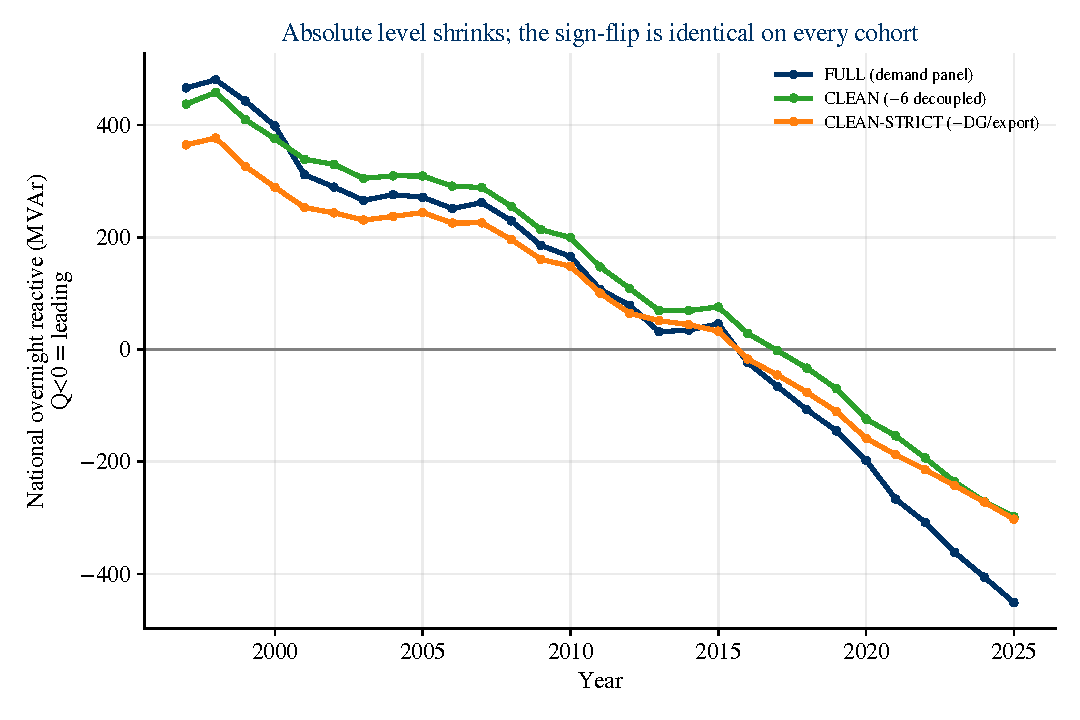
\includegraphics[width=0.90\columnwidth]{01_clean_cohort.pdf}
\caption{The trajectory is robust to removing contaminated grid exit points: the
national overnight total on the full demand panel and on the clean and
clean-strict cohorts (the latter also removing distributed-generation, ``DG'',
and net-export sites). The absolute level falls as large decoupled nodes are
removed, but every cohort makes the same lagging-to-leading crossing, and the
per-MW drift intensity is unchanged across cohorts ($-0.0175$, $-0.0178$,
$-0.0180$~MVAr/MW/yr). The contamination inflates the level, not the direction or
intensity of the drift.}
\label{fig:clean}
\end{figure}

% ======================================================================
\section{Decomposition: Demand vs Network}
% ======================================================================
The policy-relevant question is how much of the drift is the network's own cables,
which inject leading reactive power as a distributed capacitance, and how much is
the changing make-up of electricity demand itself: the retreat of inductive plant
(simple motors) and the accumulation of power-electronic equipment (LED lighting,
switch-mode supplies, heat pumps and other variable-speed drives). We call the
second part \emph{organic}: it is in the load fleet, not the wires. If the drift
were mostly cables it would be a familiar network-planning problem; if it is mostly
the demand fleet it is structural, nationwide, and outside any single network's
control. We approach the question three ways; the two statistical methods share a
common underground-cable proxy, while the physics-based method fits no cable
coefficient and is independent of both. What the demand-side component physically
\emph{is}---the question the decomposition leaves open---is taken up in
Section~V.

\subsection{Method 1: a clean-cohort contrast}
History handed us networks at opposite ends of the cable spectrum. Some
distribution businesses are almost entirely overhead line and have almost no
underground cable; overhead line injects little leading reactive power, so these
networks have almost no cable contribution. If their overnight reactive power still
drifts leading, that drift can only be the demand fleet. We compare reactive power
per MW of load (so network size cancels), load-weighted within each cohort
(larger sites count proportionally more), for
networks at or below 12\% underground (\emph{clean} in this method's sense:
almost cable-free, distinct from the decontaminated cohorts of Section~III-B)
against networks at or above 40\% underground (cable-rich), shown in
Fig.~\ref{fig:methods}(A).

\begin{figure*}[!t]
\centering
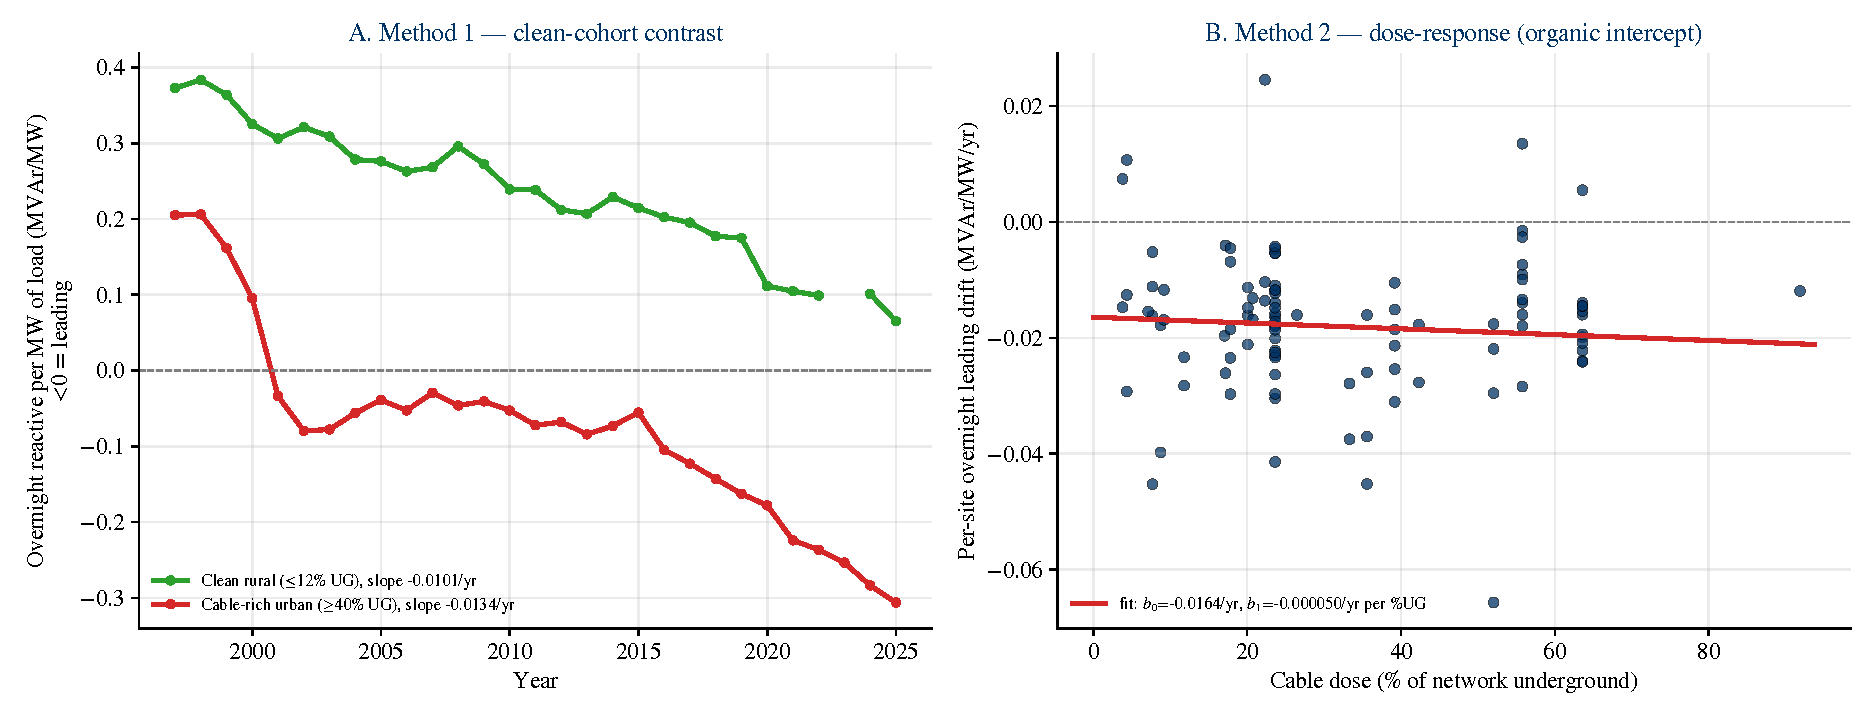
\includegraphics[width=0.78\textwidth]{02_methods.pdf}
\caption{The two statistical methods. (A) Method 1, the clean-cohort contrast:
even clean rural networks (at most 12\% underground, so almost no cable charging)
drift leading per MW of load, isolating the demand-side component; cable-rich
urban networks (at least 40\% underground) drift slightly faster and cross
further into leading. The slope ratio implies roughly 75\% of the cable-rich
cohort's drift is demand-side (64--90\% across attribution, cable-intensity, and
panel definitions; Table~\ref{tab:triangulation}). (B) Method 2, the validated dose-response: each
point is a GXP's overnight leading drift against its cable dose (its network's
percentage underground). The drift is
already strongly leading at zero cable (the fitted intercept $b_0$, the organic
demand-side signal); the slope with cable is weakly identified (its interval
crosses zero), so the exact organic share is not pinned by statistics alone.}
\label{fig:methods}
\end{figure*}

The clean cohort drifts from $+0.373$ to $+0.065$~MVAr/MW (slope $-0.0101$/yr),
ending near balanced; the cable-rich cohort drifts from $+0.205$ to $-0.306$~MVAr/MW
(slope $-0.0134$/yr), crossing well into leading. The ratio of slopes
($0.0101/0.0134 \approx 0.75$) puts the
demand-side share of the cable-rich cohort's drift at about 75\%, cable the
remaining 25\%. The reading rests on two assumptions the split depends on, stated plainly:
that the organic per-MW drift is common across the cohorts (to the extent urban
load fleets modernise faster than rural ones, the cable share is overstated), and
that the at-most-12\%-underground cohort carries no material cable term (to the
extent it does, the demand share is overstated); the two possible violations pull
the split in opposite directions.

Three further caveats bound the ratio.
Schedule~9c offers two circuit-length tables that differ by a few points of
\%UG (percentage underground)
for cabled networks, and Method~1 gives about 75\% under the ``total length for
supply'' table against about 69\% under the ``by operating voltage'' table
(Unison sits on the 40\%-underground boundary at 39--45\% across averaging
choices, so its cohort membership, though not the load-weighted ratio, turns on
the same choice). A separate circuit-length series taken over all grid exit
points rather than the balanced panel yields a wider, roughly 90/10 reading.
And the ratio moves with how the grid exit points that
changed network (Section~II-D) are attributed: carrying each site's successor
cable dose throughout (the wires being physically continuous), rather than
entering it in the cable-rich cohort only once its successor company discloses,
steepens the cable-rich drift to $-0.0159$/yr and moves the split to about 64\%
demand; the clean cohort contains no such site and is identical under every
attribution, so the organic direction is untouched.

The \emph{direction} is therefore robust while the \emph{exact ratio} is not, which is why we treat Method~1's
ratio as a hypothesis and bring two further methods. The contrast is also robust to
the metering contamination of Section~II-E:
the cable-rich cohort contains the two decoupled Christchurch nodes
(Islington and Bromley), and removing them softens the cable-rich drift to
$-0.0129$/yr and moves the split to about 78\% demand, 22\% cable---so the
contamination, if anything, overstated the cable share, and removing them
strengthens the demand reading. And although cable is the minority of the drift, it is the marginal factor
that tips a network from balanced into net-leading: the clean cohort ends near
balanced while the cable-rich crosses into leading, so cable intensity shapes
\emph{where} overvoltage appears first even though demand composition drives the
trend.

\subsection{Method 2: a validated dose-response}
The second method asks whether the networks with more cable drift faster. Each
GXP is reduced to one number---the Theil--Sen slope of its overnight reactive
power through the 29 years, scaled by its own typical size---and those per-site
drifts are then fitted against the site's \emph{cable dose}, the percentage of
its network that runs underground. The line has two coefficients, and only one of them is this paper's
result. At zero cable there is no cable charging, so any drift remaining at that
end of the line must come from the demand: the intercept $b_0$ is the organic
drift. The slope $b_1$ is the extra drift per added point of underground---the
cable contribution.

Two features of the fit follow from how the dose is recorded. Cable dose is a
property of the \emph{company}, so every site in a network carries the identical
value and the sites are not independent. The model therefore lets each company
sit at its own baseline (a random intercept per company), and the uncertainty
comes from a \emph{cluster bootstrap}: the fit is re-estimated on thousands of
datasets drawn at random, with replacement, from the data itself, and the
reported interval is the spread of those answers---drawing whole companies
rather than single sites, so that the dependence is carried into the
interval. The interval is computed by refitting within each company-resample by
ordinary least squares; refitting the mixed model instead leaves it unchanged at
the reported precision.

Before any use on the real data, the estimator was validated on synthetic panels
with known planted answers, built on the real company structure and real cable
doses and run through the identical machinery in two scenarios (a planted cable
effect, and none); the full protocol and results are in the accompanying
notebooks. The validation licenses a specific and limited claim. The estimator
recovers the sign and magnitude of the organic drift reliably in both regimes.
It point-identifies (pins to a single number) the organic \emph{share} only when
the cable effect is itself identified, and the reason is arithmetic: that share
is $b_0/(b_0+b_1 d)$ at dose $d$, which puts $b_1$ in the denominator. A precise
numerator over an uncertain denominator is an uncertain ratio, so on the real
data the share cannot be pinned even though $b_0$ is, and we rest no magnitude on
this method. Line-fitting can neither manufacture a split here nor, with a cable
effect indistinguishable from zero, pin one; the magnitude falls to Method~3.

On the real data (Fig.~\ref{fig:methods}(B)), the organic drift is $b_0=-0.016$/yr
(95\% CI $[-0.021,-0.010]$), leading in 100\% of bootstrap resamples: unambiguous
and dominant. The cable slope is $b_1=-0.00005$/yr (95\% CI
$[-0.00037,+0.00012]$), which crosses zero---weakly identified, because cable dose
is a company-level trait with only about 23 distinct values---so we deliberately
publish no tight interval on the share (read across the cable range, the point
estimate runs from 93\% at the median dose to 78\% at the most cabled networks,
consistent with 100\%; the point estimate is the single best-guess number
before any range is put around it). Three robustness checks hold: adding capacitor intensity
to the fit as a control (the cable effect read at fixed capacitor intensity)
moves $b_0$ by only about 10\% and leaves it strongly leading
(consistent with the static-to-declining capacitor fleet of Section~VI-B); the
low correlation between cable dose and distributed-generation intensity ($-0.22$)
indicates the organic signal is not an artefact of where embedded generation
sits; and restoring the four sites dropped for want of a disclosing owner in
the Section~II-D mapping under their successor's cable dose moves $b_0$ by
under 1\%.

A fourth check replaces the dose measure altogether: refitting with each
network's computed charging intensity as the dose---Method~3's physical
$\omega C V^2 \ell$ (Section~IV-C) summed and taken per MW of maximum
demand---moves $b_0$ only from $-0.0164$ to $-0.0178$/yr, with the cable term
still crossing zero. The two dose measures are in fact \emph{negatively}
correlated across networks ($r=-0.23$): the near-all-overhead rural networks
carry far more circuit length per MW of demand (69--89~km per MW at the
overhead extreme against 9--11 at the most-cabled) and end up with \emph{more}
computed charging per MW than the most-cabled urban networks, so percentage
underground is in part an urban-density measure rather than a
charging-intensity one. That two nearly opposite dose definitions return the
same organic conclusion is a stronger robustness statement than either alone.
(The charging-intensity dose shares its per-MW denominator with the per-site
drifts, which can bias the cable slope but not the zero-cable intercept; no
reading here rests on the slope under either dose.)

Method~1's urbanisation confound applies here too, and in the same
direction: the cable dose is a company-level trait, so if urban fleets modernise
faster than rural ones some of that difference loads onto $b_1$ rather than
$b_0$, overstating cable and understating the organic term. The bias is
conservative for the reading we take.

\subsection{Method 3: first-principles charging physics}
The third method computes the network contribution directly from physics, with no
fitted coefficient, so it sidesteps the weak-identification problem entirely. Any
energised length of cable or line behaves as a distributed capacitance and injects
a fixed leading reactive power $Q=\omega C V^2 \ell$, where $\omega=2\pi\cdot
50$~rad/s, $C$ is capacitance per km, $V$ the operating voltage, and $\ell$ the
length. Underground cable has far more capacitance per km than overhead line. Using
the published overhead and underground kilometres at each voltage from
Schedule~9c, textbook per-km capacitances with an explicit $\pm 35\%$ band, and a
band-by-band sum (charging scales with $V^2$, so high-voltage lines dominate), we
compute the physical charging per network per year and subtract it from the
measured overnight reactive power; the remainder is organic
(Fig.~\ref{fig:physics}).

The operating voltage in each band is its \emph{nominal} value, held constant
across the record, and since charging scales with $V^2$ a systematic drift in
operating voltage would move the computed term and land the difference in the
residual. Three things bound it. First, where the charging sits: 77\% of the
computed 2025 total is at or below 33~kV (Table~\ref{tab:bands}), on the
distribution side of the grid exit point transformer, where the on-load tap
changer holds voltage to a setpoint rather than letting it follow the transmission
system---so most of the term sits behind a regulator, not adrift. Second, the
direction of the documented adaptation: distributors facing rising light-load
voltage have tapped \emph{down} and re-tapped distribution transformers, which
lowers the true charging below the computed value and makes the residual, and
hence the organic share, \emph{conservative}. Third, the size: re-running the
whole decomposition under a per-year voltage ramp $k(t)=(1+g(t-2013))^2$ applied
to the computed charging moves the central organic share by $-7.8$ percentage
points for a 5\% rise across the window and $+7.4$ for a 5\% fall, and a sustained
rise of 4.2\% (0.35\% a year for twelve years, against a statutory band of
$\pm 6\%$ for most of the record) would be required to carry the share below the
75\% floor of the physical band. The two mechanisms also pull against each other:
a rise on the transmission side is what provokes the tapping down on the
distribution side. The band is set to span published per-km capacitance
values across common distribution cable constructions and cross-sections, and it is
carried through to the result rather than quoted and dropped. The organic remainder is a residual, and we name the principal further terms
it absorbs: transformer magnetising reactive power (lagging, so static or growing
alike mask leading), series-reactance absorption (minimal at light load, and
rising over the window with overnight demand rather than falling), and the
distribution capacitor fleet (static-to-shrinking, Section~VI-B, so its change
also removes leading). Each is either second-order overnight or biases the
residual toward lagging, so reading the residual as the demand-side drift is
conservative in respect of these terms. It is not an exhaustive accounting: the Method~3 footprint carries no
decoupled-node screen, so any embedded generation running a night-time reactive
mode also sits in the residual. We therefore remove those sites rather than only
naming them. Re-running the decomposition on the decontaminated footprint puts the
organic share of the drift at 82\% with the six decoupled nodes of Section~II-E
removed, and at 89\% (physical band 86--93\%) once every steady-generation and
net-export site is removed as well. Charging is disclosed per network while the
flags are per grid exit point, so each network's charging is scaled by its
retained share of overnight demand; dropping whole networks instead leaves too
few to read at the strict screen.

The direction is what this check delivers: every screen that removes embedded
generation moves the share \emph{up}, so the headline figure is not inflated by
those sites and the conservative reading survives this term as well. \emph{We do
not restate the headline on this basis.} The decontaminated footprint is a
smaller and different sample rather than a better measurement of the national
quantity---those sites are real grid exit points carrying real reactive flow at
the boundary---and the physical bands overlap, so the shift is not resolvable
against the $\pm 35\%$ capacitance uncertainty that dominates this method. The
check licenses reading $\sim$80\% as conservative, not as understated.

\begin{figure*}[!t]
\centering
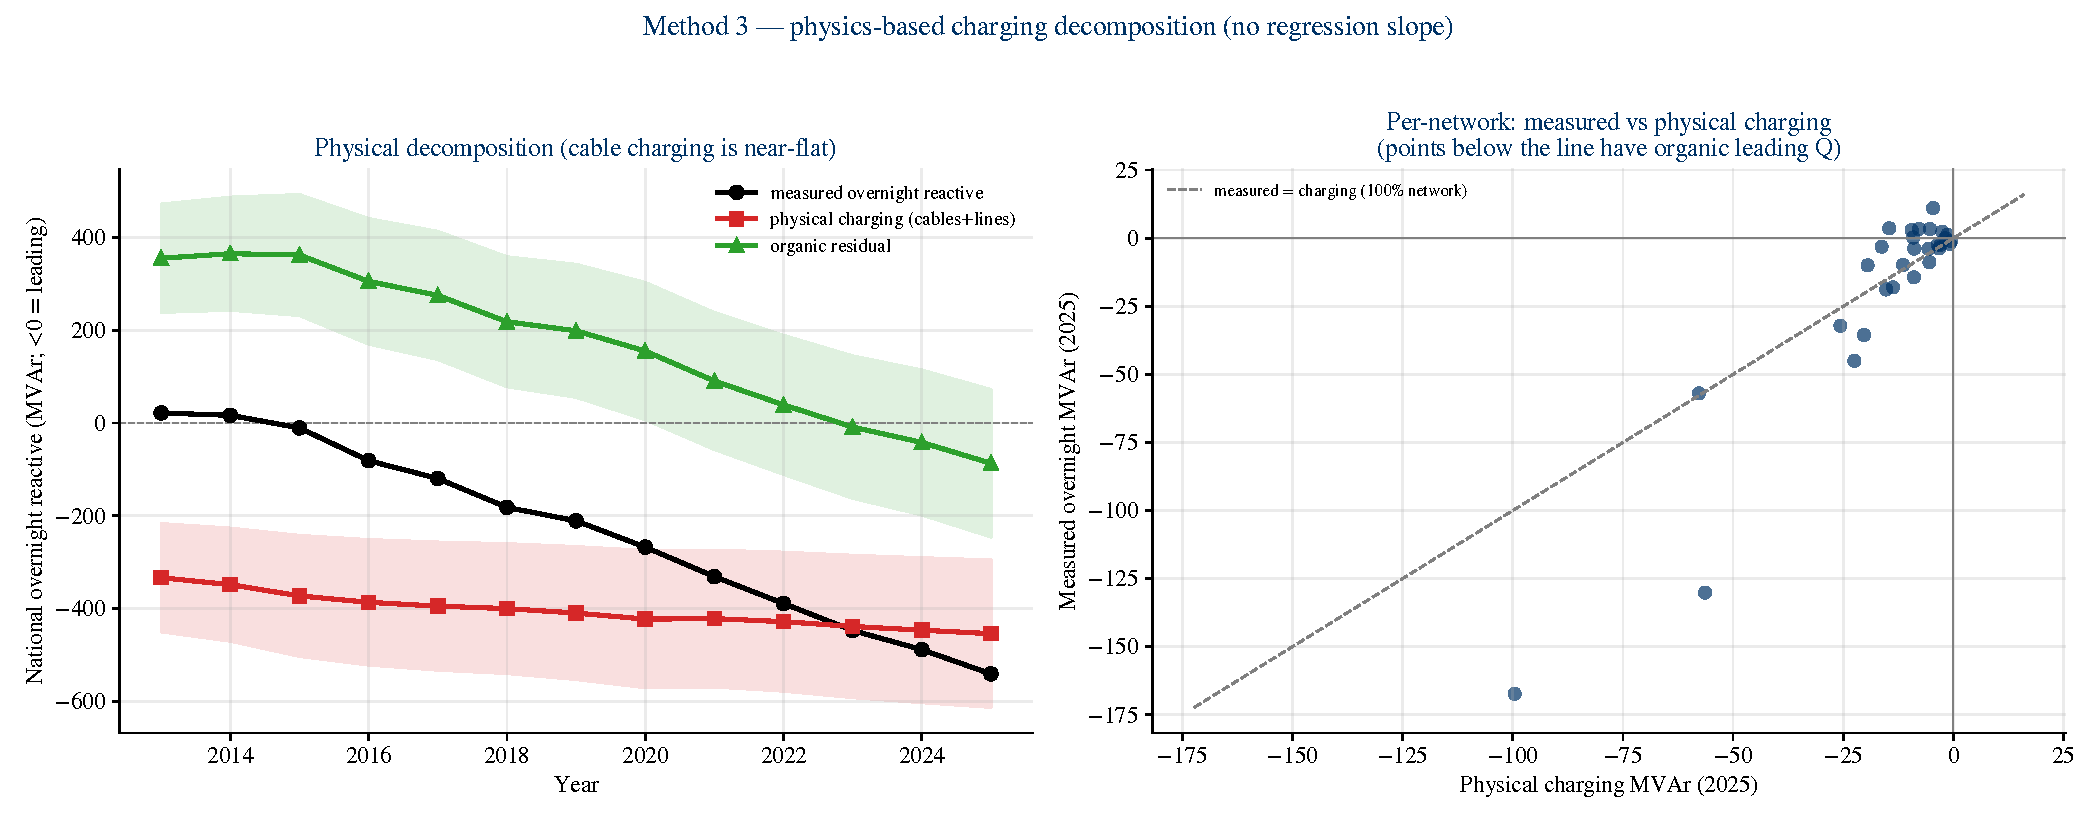
\includegraphics[width=0.74\textwidth]{03_physical_charging.pdf}
\caption{Method 3, the physics-based decomposition over the all-network footprint
(2013--2025, the years with consistent Commerce Commission circuit-length
disclosures, from which the charging is computed). The physical cable
and line charging (red, with the $\pm 35\%$ band shaded) is near-flat because cable
length grows slowly, so almost all of the worsening trend in the measured overnight
reactive power (black) is the organic residual (green). The drift is about 80\%
organic (physical band 75--88\%). The right panel shows, per network, that most
points lie below the unity line, i.e.\ carry organic leading reactive power beyond
their charging.}
\label{fig:physics}
\end{figure*}

Over 2013--2025 the measured overnight reactive power drifts at $-49.9$~MVAr/yr
across all demand networks, of which the physical charging contributes only
$-9.2$~MVAr/yr (cable length grows slowly) and the organic residual $-40.7$~MVAr/yr.
The organic share of the \emph{drift} is therefore about 80\% (physical band
75--88\%). Because this method fits no cable coefficient, it is independent of
the two statistical methods; the division of labour is collected in
Section~IV-D. The
window is set by the data: the disclosed circuit kilometres it runs on
(Section~II-D) are recorded consistently only from 2013, so the
physics decomposes the 2013--2025 drift, about 45\% of the record; extending the
$\sim$80\% share to the full 29 years is an inference, supported by the
direction-consistent statistical methods (which do span the full record) and by the
slow growth of cable length, not a second measurement. We
stress that this all-network footprint rate ($-49.9$~MVAr/yr,
2013--2025) is a different dataset from the balanced panels of Section~III
($-31.1$~MVAr/yr on the 123-GXP demand panel; $-30.3$ on the 132-GXP panel,
1997--2025) and from a separate cable-correlation analysis of the
same public records, reported in the accompanying notebooks ($\approx
46$~MVAr/yr); these measure different things
over different samples and are not interchangeable.

\begin{table}[!t]
\caption{Computed Physical Charging by Voltage Band, 2025 (Central
Capacitance Values, on the Footprint of Fig.~\ref{fig:physics})}
\label{tab:bands}
\centering
\renewcommand{\arraystretch}{1.18}
\begin{tabular}{@{}lrrr@{}}
\toprule
\textbf{Band} & \textbf{UG km} & \textbf{OH km} & \textbf{Share of charging} \\
\midrule
6.6--11~kV            & 17,365 & 67,729 & 41\%  \\
33~kV                 &  1,747 &  6,983 & 29\%  \\
50 \& 66~kV           &    118 &  2,406 & 12\%  \\
$>$66~kV              &     52 &    537 & 11\%  \\
22~kV                 &    795 &  3,488 & 6\%   \\
Low voltage ($<$1~kV) & 31,884 & 23,552 & 0.2\% \\
SWER                  &     24 &  3,271 & 0.1\% \\
\bottomrule
\end{tabular}
\end{table}

Table~\ref{tab:bands} breaks the computed charging out by voltage band, and
it is why the band-by-band sum matters. Underground cable carries about 76\%
of the computed charging and overhead line the rest, with the total rising
from 335 to 454~MVAr over 2013--2025 on this footprint. The low-voltage row
is the instructive one: LV is by far the largest underground
category---31,884~km, more than the 11~kV band's 17,365---and contributes
0.2\% of the charging, because charging scales with $V^2$. A
single-average-voltage treatment would misattribute it badly; the 6.6--11~kV
and 33~kV bands, which carry most of the underground kilometres that matter,
contribute about 70\% between them.

A separate and more uncertain question is the composition of the leading reactive
power \emph{standing on the network today} (the level, as opposed to the drift). On
the level the physics points the other way: a large, near-static cable and line
charging baseline has always been present, and what changed is that the organic
demand shifted from lagging---which used to mask the charging---toward leading,
which no longer does. Today's net leading reactive power is then mostly
long-standing charging \emph{revealed} rather than newly created. The exact level
split has a wide physical band and we do not quote a precise share for it; the level
is a distinct, weaker claim and must not be confused with the drift result. We carry
this only as the qualitative ``uncovered charging'' reading that informs
Sections~VI and VII.

\subsection{Triangulation}
Table~\ref{tab:triangulation} collects the three methods, which play different roles
and are not all independent: Methods~1 and 2 both rest on the same underground-cable
proxy, whereas Method~3 fits no cable coefficient at
all. All three, though, consume the same Schedule~9c circuit-length
disclosures---cohort definition and dose in Methods~1 and 2, the length $\ell$
in Method~3---so agreement among them cannot diagnose a systematic kilometre
error, which would move all three coherently; under-counted cable would push
every method toward the demand side.

The reading follows that division of labour. The \emph{direction} is
robust and identified: the organic drift is leading in 100\% of bootstrap resamples
while the cable contribution to the drift is not statistically distinguishable from
zero, and together these imply the drift is dominantly demand-side. The
\emph{magnitude} is carried by the physics: the first-principles charging calculation,
which fits no cable coefficient, puts the organic share at about 80\% (physical band
75--88\%). The two statistical methods are directionally consistent but, because the
marginal cable effect (the extra drift per unit of cable) is not identified at
the few company-level cable values
available, do not themselves pin the share. We report the drift as dominantly organic
and do not claim a point-identified split. Cable is the minority of the drift but the
marginal factor in where net-leading territory is reached first.

A cross-sectional check agrees: ranking the demand grid exit points by how
leading they now are, the
most-leading group is not the most-cabled---the sites with the steepest drift and
the highest leading fraction sit at roughly half the cable intensity of the
most-cabled group, and the gap widens further when the decoupled Christchurch
nodes of Section~II-E are removed---so cable cannot be what drives the
deepest-leading behaviour, independently confirming the demand-side reading (the full cross-sectional
typology is in the reproducibility notebooks). The three methods share a subject---the \emph{rate} at which the
overnight reactive power moved---and none of them describes the standing level.
Figure~\ref{fig:physics} separates the two, because the distinction carries the
practical reading: the distribution network's charging is the larger part of the leading reactive power present tonight, and the demand is the larger part of why that total has moved.

\begin{table}[!t]
\caption{Three Decompositions of the Drift}
\label{tab:triangulation}
\centering
\renewcommand{\arraystretch}{1.18}
\begin{tabular}{@{}p{0.27\columnwidth}p{0.24\columnwidth}p{0.37\columnwidth}@{}}
\toprule
\textbf{Method} & \textbf{Establishes} & \textbf{Organic share of drift} \\
\midrule
1: clean-cohort contrast (cable proxy) & direction (shares the cable proxy with 2) & $\sim$75\% (78\% with contaminated nodes removed; 64--90\% across attribution, cable-intensity, and panel definitions) \\
2: dose-response (cable proxy) & direction / dominance & $\geq$78\%, consistent with 100\% (cable term not pinned by the data) \\
3: charging physics (no fitted cable term) & \textbf{magnitude} & $\sim$80\% (physical band 75--88\%) \\
\bottomrule
\end{tabular}
\end{table}

% ======================================================================
\section{The Demand-Side Term Identified: A Standing Shunt Term Behind
Connections}
% ======================================================================
The decomposition attributes the drift to the demand fleet; it does not say what
in the fleet is doing it. Two measured properties narrow the answer, a specific
physical candidate follows from them, and a scaling test probes the candidate's
sharpest prediction.

\subsection{Load-independent, around the clock}
First, the drift is load-independent. Over the 2013--2025 window we summarise
each grid exit point passing the full contamination screen (the clean-strict
criteria of Section~III-B, applied here to all sites metered in the window
rather than to the 29-year balanced panel) by robust annual medians on wider
windows than the Section~II features (trading periods 1--12, midnight--06:00,
and 35--39, 17:00--19:30). On the 114 such grid exit points with both endpoints
metered, the median per-site change in reactive power is $-2.25$~MVAr overnight
and $-2.42$~MVAr at the evening peak (median per-site ratio 1.06), while
evening-peak load was essentially flat (median change $+2.9\%$). A change in how
the connected load draws reactive power while operating would scale with the
load operating---far larger at the peak than at 03:00---and so would the
load-proportional metering bias bounded in Appendix~A, whose spurious term goes
as $P\sin\beta$. A near-equal deepening around the clock is instead the
signature of a \emph{standing shunt term}: always energised, indifferent to
what the load is doing. It also reconciles the diurnal structure of
Fig.~\ref{fig:traj}: the two windows drift in parallel, and net-leading surfaces
overnight first because the standing component is netted against more lagging
load at the peak.

The peak/overnight comparison carries a second, quantitative reading that the
load-independence argument does not need but which bounds it. A purely standing
shunt term scales with $V^2$, and evening-peak voltage runs \emph{below} overnight
voltage, so such a term should deepen slightly less at the peak, not more. Taking
equal deepening as the conservative null, the measured excess at the peak
($-2.42$ against $-2.25$~MVAr) is $0.17$~MVAr, or about 7\% of the peak change:
an upper bound on the load-proportional component of the whole movement. Allowing
the peak voltage to run 2--5\% below the overnight value raises that bound to
11--16\%. It is a bound and not an estimate---the load-proportional part could be
zero---but it is a bound the record supplies for free.

\subsubsection*{The measured quantity is a net shunt term}
What this test identifies is the \emph{net} standing shunt term, and the
distinction governs everything claimed after it. A standing shunt
\emph{inductance} has the same three signatures as a standing shunt
\emph{capacitance}: it is load-independent, it is permanently energised, and its
injection scales with $V^2$. Writing the net as $Q_L-Q_C$, the record delivers
$Q_L-Q_C$ in every year and never $Q_L$ and $Q_C$ separately, so a movement of the
net is consistent with capacitance added, inductance removed, or any combination.
Fig.~\ref{fig:icp}B makes the point concrete: the per-connection term stands at
$+41$~VAr (inductive) in 2009 and reaches $-262$~VAr by 2025, a movement of
303~VAr whose two limbs the measurement does not resolve.

Both limbs were moving inside the window, and the inductive one is not a
second-order correction. The classes that count are those permanently energised
at 03:00, which is a much narrower set than the fleet at large---anything switched
off overnight contributes to the evening peak and not to the headline window, so
residential lighting and its halogen transformers drop out of the inventory
whatever their installed base. What survives that filter:
\begin{itemize}
\item \emph{Linear transformer supplies.} A small mains-frequency transformer with
  a bridge rectifier draws its magnetising current whenever it is plugged in, and
  small cheap transformers magnetise poorly: no-load current of 20--40\% of rated
  is typical, so a 6~VA unit stands at roughly 1--3~VAr inductive. Its
  switch-mode replacement, if it carries an X-capacitor at all, stands at up to a
  few VAr \emph{capacitive}. The substitution swing is therefore 2--6~VAr per
  device rather than the 2--4~VAr the capacitance-only estimate of Section~V-B
  credits---the estimate counts the capacitor added and not the inductance
  removed. Survivorship works the same way: the units that last longest are the
  ones nobody has a reason to touch, and those are disproportionately the
  permanently energised ones (doorbell and alarm supplies, gate and garage
  controllers, intercoms, low-voltage garden lighting), several of them wired
  rather than plugged and retired on the building cycle. The stock's inflow
  effectively stopped in the late 2000s, but the retirement rate of a stock with
  no inflow peaks a service life later, not when the inflow stops.
\item \emph{Magnetic-ballast lighting left on overnight.} Street lighting and
  commercial security, stairwell and display lighting run on wound ballasts at
  power factors near 0.5 lagging, are energised through exactly the measurement
  window, and converted to light-emitting diodes across the window.
\item \emph{Always-on motors.} Shaded-pole and split-phase compressors, extract
  fans, circulation and pool pumps, moving to inverter drives.
\item \emph{Distribution transformer magnetising reactive power.} Named in
  Section~IV-C as a residual absorber, it belongs here too, because it has the
  same identification signature as the claimed device fleet: standing,
  connection-scaling, and inductive. A renewed fleet magnetises less.
\end{itemize}
A retirement moves the net exactly as an addition does, and neither the level nor
the connection-scaling test can tell them apart. We therefore report the net term
throughout and advance the device layer of Section~V-B as a candidate for its
\emph{capacitive limb alone}, leaving the split as stated future work
(Section~VIII). Two routes to it are identified there: the standing power factor
measured at the start of the record, which anchors the inductive limb at one
endpoint, and the frequency sensitivity of the aggregate, which returns
$Q_L+Q_C$ where the level returns $Q_L-Q_C$.

\subsection{A physical candidate: the mandated EMC filter}
Second, the term must live behind essentially every connection, because
the drift's reach is near-universal across grid exit points (Section~III-B). We
therefore advance a specific physical candidate, labelled plainly as a
hypothesis: the electromagnetic-compatibility (EMC) filter that practically
every mains-connected electronic product is required to carry. A switched-mode
device chops current at tens to hundreds of kilohertz, and conducted-emission
limits (the international CISPR limits~\cite{cispr32}, covering roughly
150~kHz--30~MHz, a condition of sale in most jurisdictions, New Zealand
included; the same obligation reaches household appliances through CISPR~14-1,
on a lineage older still, and variable-speed drives through IEC~61800-3) oblige
its manufacturer to stop that noise at the appliance's own
terminals; the universal compliance solution is a passive filter directly
across the mains input.

Its elements carry safety-class names~\cite{iec60384_14} from where they
connect: \emph{X-capacitors} bridge line and neutral---the one position where
a capacitor is permitted to be large (typically 0.1--2.2~$\mu$F), because a
short circuit there is an overcurrent event the appliance's fuse clears rather
than a shock hazard---while \emph{Y-capacitors} run from the conductors to
earth, where a short would electrify the chassis, so they must be built never
to fail short and are held to nanofarads by touch-current limits; a
common-mode choke completes the filter (Appendix~B).

At 50~Hz the filter's only material injection is
the X-capacitance, which sits across 230~V drawing pure leading current
whenever the plug is live: 0.1--1~$\mu$F injects 1.7--16.6~VAr, around the
clock, because the filter sits ahead of the rectifier and of any standby
logic---it must, since the noise it suppresses would otherwise leak even in
standby. At 230~V the arithmetic is $Q=\omega C V^2$: 0.1, 0.47, 1, and
2.2~$\mu$F inject 1.7, 7.8, 16.6, and 36.6~VAr respectively. The fleet is one
worldwide design, so the capacitance is chosen once and the mains it lands on
sets the draw: the same microfarad that injects 16.6~VAr here injects 5.4~VAr
on North America's 120~V, 60~Hz mains and 3.1--3.8~VAr at Japan's
100~V---roughly three times the standing draw per device at 230~V as in North
America, and four to five times Japan's. The Y-capacitors
are not quite silent---where the appliance is earthed, the line-to-earth
element injects too---but at nanofarad scale it is under a per cent of the
X-capacitor beside it, and the numerous small always-connected devices are
double-insulated with no protective earth at all (Appendix~B). Counting X alone
biases the estimate very slightly low.

Commercial equipment carries larger input filters: a variable-speed
drive holds tens of VAr and upward, energised wherever the installation is
left connected. The regulatory structure makes the accumulation one-way: one
instrument drives the capacitance into practically every product---the filter is
the universal compliance solution, not a named requirement---while, as
Section~I-A
noted, no instrument bounds its fundamental-frequency injection---and a larger
X-capacitor is generally the cheaper route to compliance. The filter's own
earth-side element shows what recognition of an aggregating current looks
like: leakage sums across everything sharing a protective conductor, and the
regime bounds it at both scales---per device, through the touch-current
limits that hold Y-capacitance to nanofarads, and per installation, where
wiring rules hold a protected circuit's accumulated standing leakage to a
fraction of its residual-current device's rating~\cite{bs7671}. The
X-capacitance's fundamental-frequency current aggregates just as
surely---tens of devices behind a connection, whole fleets behind a grid exit
point---but each device is certified alone, against a standardised artificial
mains network, and the sum is, as far as we are aware, bounded at no scale by
any instrument (Appendix~B).

New Zealand's compliance instrument even encodes the two populations: since at least 2004 the
EMC notice has assigned products incorporating switched-mode power supplies to
a conformity level requiring a test report, while leaving wire-wound
mains-frequency transformers at the lowest level~\cite{rsm_emc2019}. Nor is
the mandate the newcomer: the conducted-emission requirement has been the
sole route to the European market since the start of 1996~\cite{eu_emc1989}
and a condition of sale in New Zealand since at least 2001, so the term's
youth is the fleet's, not the rule's---what scaled through the 2000s and
2010s is the switched-mode population the rule reaches, while the wire-wound
fleet those classes displaced carried no filter at all.

The hypothesis is disciplined by what it excludes: the large DC-link capacitor
behind the rectifier makes no standing fundamental-frequency injection, being
recharged through rectifier conduction pulses only while the device draws
power; motor-run
capacitors sit in series with the motor's auxiliary winding
and are disconnected with it; and rooftop solar inverters contribute almost
none overnight (the isolation relay strands the converter-side filter
capacitors, leaving only a small grid-side element).

The last of those exclusions carries the most weight and is the one most open to
challenge, since inverter topologies differ in where the anti-islanding relay sits
relative to the mains filter and the photovoltaic fleet grew substantially inside
the headline window. It is therefore bounded rather than asserted. Schedule~9e
records distributed-generation connections made each year; summed over 2013--2025
the count is about 72,000, itself an over-count for photovoltaics because the
series covers all distributed generation. At the top of the datasheet range for a
mains filter (2.2~$\mu$F, 36.6~VAr) the whole fleet reaches 2.6~MVAr, or 0.7\% of
the 369~MVAr swing those grid exit points recorded. Granting the objection in
full---the entire converter-side filter of a residential inverter, of order
10~$\mu$F, left energised on the grid side of the relay at every one of those
connections---reaches 11.9~MVAr, about 3\%. Night-time reactive modes at zero
active power would sit on top of that, and are a real and growing mechanism
(Section~II-E flags exactly this at transmission scale), but they are dispatched
rather than standing, and would not reproduce the connection-scaling signature of
Section~V-C on a fleet that reaches under a fifth of connections.

A bottom-up order-of-magnitude estimate---roughly two million households, each with 20--40
permanently connected filter-carrying devices at 2--4~VAr (the population above
roughly 25~W: network, audio-visual, computing, and appliance electronics;
published reference designs at or below 20~W carry no X-capacitor at all, and
below about 25~W its presence is design-dependent rather than general
(Appendix~B); roughly
80--320~MVAr in aggregate), plus a commercial and
industrial fleet of the same order---puts the national standing total at roughly
150--600~MVAr, or 100--200~VAr per household as the central band.

Sizing its most recognisable member bounds the composition: heat pumps were used in 66.8\% of
occupied private dwellings at the 2023 census, up from 47.3\% in 2018---an
adoption jump inside the study window, mostly at existing
homes~\cite{ehinz_heating}---implying, at 1.2--1.6 units per equipped home,
roughly 1.6--2.1 million residential units. Reference-design filter values for
the outdoor units---the largest per-device contributors we found---are
1.4--2.0~$\mu$F each (23--33~VAr), putting the class at roughly 37--69~MVAr.
Against the 80--320~MVAr residential envelope that is of order a quarter at
central values: a material slice, but a minority, so the bulk of the standing
term belongs
to the far more numerous small supplies. Because the filter, unlike the heating
duty, is energised year-round, the slice is also consistent with the drift's
winter--summer invariance (Section~III-B); a heating-season mechanism would not
be.

The per-device values are physics and datasheet-grade figures, not New Zealand bench
measurements---reference designs rather than teardowns of shipped New Zealand
product---and the device counts are estimate arithmetic rather than a New
Zealand census; we grade the attribution accordingly (component-level basis in
Appendix~B). The 20--40 band is anchored by
the standby literature: 19 standby appliances per household across ten
Californian homes in 2000~\cite{ross_meier2000}, and about 39 products per
household in 2000 rising to 67 by 2005 in the Australian intrusive
surveys~\cite{edlington2006}. The estimate's value is
that it makes two testable predictions: the national scale of the drift,
and---because the fleet lives behind consumer connections---that the drift
should scale with the number of connections served, with nothing left at zero
connections.

The first prediction is met at the order-of-magnitude grade the estimate
carries. Summed across the same 114 grid exit points, the median overnight
reactive power moved from $+188$~MVAr (net absorbing) in 2013 to $-182$~MVAr in
2025: a deepening of 369~MVAr (summarising each site by its 99th-percentile
leading half-hour of the year, rather than its overnight median, gives
314~MVAr; the sites that deepened contribute 427~MVAr before the few that
shallowed are netted off). Those exit points serve about 1.5~million
connections, near 70\% of the national total, so the rise normalises to about
210--280~VAr per connection on the footprint that produced it (209 and 285 on
the two bracketing summaries above, 314 and 427~MVAr over 1.5~million
connections, rounded inward)---above the
estimate's 100--200~VAr per household centre rather than inside it. The gap is
expected rather than anomalous, and Section~V-C quantifies it: a connection is
not a household, since the count includes commercial and industrial connections
carrying larger filter fleets, and each connection also brings its share of
medium-voltage cable. This is a bracket, not an allocation---the estimate
bounds today's standing total, of which the twelve-year rise is the recently
added part---and it is a bracket an order of magnitude wide by construction:
what it can refute is a bottom-up estimate wrong by that much in either
direction, and this one is not.

The dose arithmetic adds a third, cross-country prediction. If the filter is
the mechanism, the per-connection drift should order across systems as
$\omega V^2$---Japan, then North America, then the 230-volt world---an
ordering that cables, heat pumps, and correction plant have no reason to
reproduce (Section~VIII). The step from arithmetic to prediction carries one substantial qualification, and
it is the reason this is offered as a test rather than a conclusion. The
X-capacitor is not sized to a reactive-power target but to attenuate
differential-mode conducted noise to a limit expressed in dB$\mu$V. For the same
output power a 120-volt input draws twice the current and presents a lower source
impedance, so the same limit demands more differential-mode attenuation, which a
designer may buy with capacitance rather than inductance---North American designs
can therefore need \emph{more} X-capacitance, not the same, which offsets part of
the $V^2$ dose. The offset is bounded by the same commercial logic that creates
the fleet: a universal-input supply (90--264~V) is designed once and sold
everywhere, and for that population the capacitance genuinely is chosen once and
the mains sets the draw. The prediction is therefore strongest for globally
traded universal-input product and weakest where a market gets its own design.

Every system in Section~I-A runs 230-volt mains, and we are not aware of an
equivalent North American measured report. We draw no inference from that: it is
an absence of measurement, not evidence of absence, and North America differs from
the systems in Section~I-A in cable intensity, feeder topology, transmission
voltage class and reporting practice as well as in mains voltage. The claim here
is priority of measurement, not of exposure. The North American record the field
does hold confirms the arithmetic rather than contradicting it: the documented
North American case of overvoltage instability is Hydro-Qu\'ebec's ``highly
capacitive'' 735-kV network~\cite{vournas2026review}---extra-high-voltage line
charging behind 120-volt outlets, exposure in the network's voltage class
rather than the mains-voltage dose. Of the two domestic predictions the
second is the more discriminating; Section~V-C tests it.

\subsection{A connection-scaling test}
Connection counts are public: the retail market-structure dataset on the same
regulatory platform records the number of installation control points
(ICPs---metered connections) behind each network supply point, monthly, from
December 2003~\cite{emi_icp}. We sum ICPs across retailers and embedded networks
to each grid exit point, take calendar-year means for 2013 and 2025, and join
them to the cohort under a documented correspondence audit, since the
registry's root-NSP attribution and the metering's exit-point boundaries are
not the same partition of the network: of the 114 sites, eight are
direct-connect industrial points with no retail registry (a steel mill, a
smelter, pulp and dairy plants), two lack a registry endpoint, one is
unresolvable, and the remaining 103 all enter; sites whose registry codes
demonstrably swap consumers with no matching movement of metered load (blocks
of up to 27,000 move between neighbouring codes) are aggregated into station
or sibling groups, giving $n=96$ panel units. The test
regresses each unit's 2013--2025 change in median overnight reactive power on
the mean connection count it serves, against three criteria that follow from
Section~V-B's estimate and are recorded in the accompanying notebooks: the
bootstrap 95\% confidence interval on the slope excludes zero; the slope lies
within 50--400~VAr per connection---the central 100--200~VAr per-household
band widened downward because a meter records the net change rather than the
gross filter capacitance added, and upward because commercial connections
ride in the same count with more than a household's fleet; and the fit
explains a nontrivial share (more than 15\%) of the cross-site variance. A
grid-exit-point-level metering artefact, with no mechanism to scale with the
connections behind the meter, predicts the mean-only model instead (the same
average change at every site).

\begin{figure}[!t]
\centering
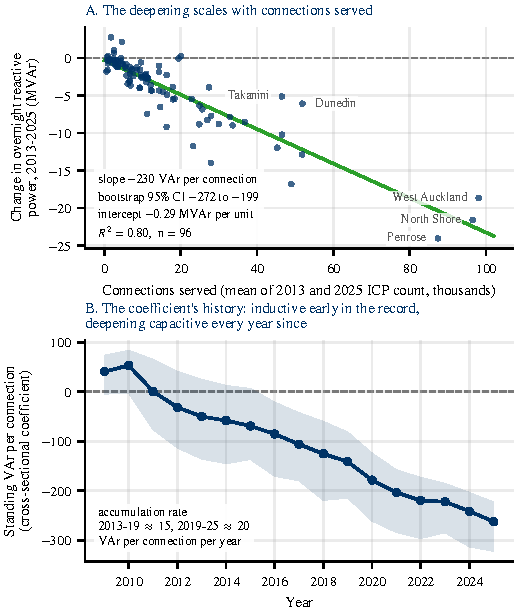
\includegraphics[width=0.94\columnwidth]{06_connection_scaling.pdf}
\caption{The connection-scaling test. (A) Each screened panel unit's
2013--2025 change in median overnight reactive power against the mean number of
connections (ICPs) it serves ($n=96$): the change deepens at $-230$~VAr per
connection (95\% CI $[-272,-199]$ resampling units, $[-313,-209]$ resampling
whole companies) with an intercept indistinguishable from zero ($-0.29$~MVAr
per unit) and
$R^2=0.80$ (80\% of the cross-unit
variance explained); deleting
any single unit moves the slope only within $[-242,-220]$, and any single
company only within $[-258,-224]$. Nothing about
a grid-exit-point metering artefact predicts an effect proportional to the
connections behind the meter. (B) The coefficient's history: the
per-connection coefficient refitted across units each year on the 92 units present throughout
2009--2025 (shaded: bootstrap 95\% CI). On the inductive side of zero early in the
record, it crosses early in the 2010s---the intervals straddle zero either side
of the crossing---and deepens every year thereafter at an accelerating rate. Sign convention: negative = added leading (capacitive) reactive power.}
\label{fig:icp}
\end{figure}

The result is Fig.~\ref{fig:icp}. The deepening scales linearly with connections
served: the slope is $-230$~VAr per connection, the fit explains 80\% of the
cross-unit variance, and a through-origin fit agrees ($-237$). The panel's 96
units serve 1.52~million connections between them and sum to 376~MVAr of
deepening, which the fitted line reproduces exactly: 348~MVAr from the slope
plus 28~MVAr from the intercept. Section~V-B's 369~MVAr is the lower
figure because it nets off the sites that shallowed and spans all 114 exit
points rather than the 103 that carry a retail registry. The coefficient
belongs to this footprint and does not scale to the national connection count,
whose connections sit partly behind excluded and contaminated exit points. Because sites
under one company share an owner and are not independent, every interval here is
reported under two resampling schemes, 4000 replicates each: resampling the 96
units independently gives a 95\% interval of $[-272,-199]$, and resampling whole
companies---the more demanding test---gives $[-313,-209]$, with a wild cluster
bootstrap rejecting the no-scaling null at $p<0.001$.

All three criteria are met, and the result is not fragile: a rank-based Theil--Sen slope agrees ($-259$), as does the
unweighted mean of the units' own per-connection rates ($-261$); deleting any
single unit moves the slope only within $[-242,-220]$ (removing the Penrose
group---PEN0221 and PEN0331; PEN1101 is excluded by the Section~II-E
screen---whose position pulls hardest on the fitted line, moves it to
$-220$, a 4\% shift with the verdict unchanged), and deleting any single
\emph{company}, which removes several high-leverage units together, moves it
within $[-258,-224]$. The high $R^2$ is not a size artefact: each unit's
own VAr-per-connection shows no material dependence on its size ($R^2=0.001$).
The mean-only artefact model loses by an Akaike information criterion (AIC)
difference of about 155, a decisive
margin on the standard model-selection score; that difference assumes
independent units, and the wild cluster bootstrap is its clustered counterpart.

A mean-only null is, however, the weak null: nobody proposes that every site
changed by the same absolute MVAr. The null that matters is site \emph{size},
because both axes scale with it, and the discriminating question is whether the
change follows connections or follows load. We therefore run the two against each
other in one specification, with each unit's overnight and evening-peak real power
built on the same parquets, windows and aggregation rule as $\Delta Q$ (members
summed per half-hour first, then the median, then the mean of the 2013 and 2025
values). Connections win on every reading. Alone, connections explain $R^2=0.80$
against 0.72 for overnight load and 0.76 for peak load, and beat both decisively on
AIC (149.0 against 184.9 and 166.9). Added to connections, neither load term earns
its parameter: $R^2$ moves 0.804 to 0.806 and AIC \emph{worsens}. In the joint fit
the connection term holds a bootstrap interval clear of zero
($-200$~VAr per connection, $[-127,-297]$) while the overnight-load term's spans it
($[-0.1,+0.1]$~MVAr/MW). The collinearity is real but not disabling: $r=0.92$
between connections and overnight load, a variance inflation factor of 6.7 on
each, below the conventional threshold at which a joint fit stops being readable.

The fit is also visibly anchored by four or five high-leverage units at the
right-hand end, so we report the leave-the-top-five-out coefficient explicitly.
Dropping West Auckland, North Shore, Penrose, Dunedin and Wellington---the five
largest by connections served---\emph{raises} the slope from $-230$ to $-261$
($[-207,-316]$, $R^2$ falling to 0.69 as the range is removed); dropping the top
ten gives $-291$ and the top twenty $-279$. The high-leverage points hold the
coefficient \emph{down}, not up, so the result is not manufactured at that end.

The intercept---what is left at zero connections---is $-0.29$~MVAr per unit
and indistinguishable from zero under every inference scheme: resampling units
gives $[-0.74,+0.21]$, resampling whole companies gives $[-0.65,+0.52]$, and
the wild cluster bootstrap retains the no-intercept null at $p=0.29$.
Aggregated across the 96 units the point estimate is $-28$~MVAr, under a tenth
of the cohort's $369$~MVAr deepening. The bottom-up estimate predicted nothing
at zero connections; the measurement meets that prediction on both
limbs. The first run under the same
criteria, on the narrower 83-site screen panel that predates the
correspondence audit, reads $-253$ (CI $[-291,-192]$, $R^2=0.77$): the same
verdict, agreeing with the audited panel to within about 10\%; we report
both, never blended. A
two-term variant separating existing connections from connections added over the
window cannot split them on this panel: the two counts are strongly correlated
across units and the added-connection term's interval spans zero, so the
accumulation-versus-growth question falls to the coefficient's history below.

The coefficient also has a history (Fig.~\ref{fig:icp}B). Refitting the
across-units regression year by year on the 92 panel units present throughout
2009--2025---each year on the standing level rather than the 2013--2025
change, so the coefficient carries the whole connection-scaling class---the
per-connection term starts on the \emph{inductive} side of the axis ($+41$~VAr
per connection in 2009, the motor-era fleet's residual signature), crosses
zero in 2012, deepens every year thereafter, and reaches $-262$~VAr per
connection by 2025. The crossing year is a point estimate: the yearly intervals
straddle zero on both sides of it, and the interval is clear of zero on the
capacitive side only from 2016, so the ramp and the post-2016 deepening are
what the data establish, not the date. The 2013--2025 movement,
$-212$~VAr per connection, reproduces the two-endpoint slope within 10\%. That
is a consistency check across two parameterisations of the same metered panel,
not corroboration by an independent route: it establishes that the result does
not depend on whether the coefficient is fitted to the endpoint change or read
off the level history.

The in-window accumulation rate rises across the window (about 15 and 20~VAr
per connection per year over 2013--2019 and 2019--2025, the 2009--2013 span
being the crossing itself)---a comparison of two window means on serially
overlapping data, reported without a test on the difference; and the
series is smooth, where a staggered metering-replacement artefact would enter
as steps (the largest single-year movements, over 2019--2021, coincide with
the pandemic years). The emergence also overlaps the 2010--2013 meter-fleet
replacement (Section~II-C), and the coincidence is worth naming: an
instrumentation change would enter as a step to a new level, not as a ramp
that crosses zero mid-record and is still deepening a decade after the
rollout ended, equally in both diurnal windows, and concentrated in the term
that scales with connections. The connection-scaling structure, in short, is not a fixture of
the network: the fleet's per-connection signature swept from inductive through
zero early in the 2010s and is still steepening on the capacitive side. We do
not attribute the crossing date to any single device class.

The inductive starting point has a domestic witness: the national household end-use project
metered real and reactive power in nine houses over 2002--2004 and found the
always-on standing load at a power factor of 0.5--0.7 inductive, attributed to
motors and ``transformer inductive loads''~\cite{heep_sr155}---the iron fleet
this record watches leave---while dismissing the era's small chargers on a
watts-only basis (``less than 0.5~W''). Two caveats travel with it: nine
non-randomly selected houses, on the project's own caveat; and its power factor
is a total rather than a displacement quantity, so at the harmonic-rich
currents of early switch-mode standby a low value need not indicate inductive
displacement, and the inductive reading rests on the load classes the project
identified rather than on a sign measurement at the fundamental. It corroborates
the starting point; it does not measure it.

Read honestly, the slope is the whole connection-scaling shunt class, not
the device fleet alone. Each connection also brings its share of medium-voltage
cable (low-voltage cable is negligible, since charging scales with $V^2$), and
commercial and industrial premises hold the one rival source of standing
capacitance at scale: power-factor-correction banks, installed against peak
lagging demand and---because correction is fitted for the lagging problem,
never its mirror---left in service overnight wherever the control is fixed or
coarsely stepped. The scale gap is the threat: a single commercial building's
stranded bank (tens of kVAr) outweighs its own device fleet twenty-fold or
more, so a slope carried by commercial connections would break the device
attribution even with the scaling law intact.

The registry separates the populations. Every connection carries an industry
classification (residential connections carry none, ANZSIC divisions A--E are
industrial, F--Z commercial), published per root NSP---the same key the
panel's counts already join on. The registry file is published as a rolling snapshot, so its history was
recovered from the Internet Archive's Wayback Machine: twenty-five
date-stamped vintages, December 2018 to October 2025, plus the live July
2026 file; a logged search found no earlier vintage anywhere, so
class-resolved history begins December 2018 (and no 2021 vintage exists).
Splitting each unit's count into its
residential and commercial-industrial parts---class counts averaged over the
eight registry year-marks---and fitting one coefficient to
each puts the residential coefficient at $-147$~VAr per connection (95\% CI
$[-240,-81]$ resampling units, $[-329,-86]$ resampling whole
companies)---on the 86\% of connections that hold no correction plant at
all---and the
commercial-industrial coefficient at $-915$ ($[-1392,-299]$ units,
$[-1288,-98]$ companies): larger per connection, as commercial device fleets
and shared cable predict. On these point estimates the two classes carry
about half the panel's 376~MVAr of deepening each---192 and 195~MVAr, a pair
that sums a little above the panel total because the two-class fit carries its
own intercept---despite the six-to-one difference in their numbers, the commercial-industrial share
running from 17 to 79\% across its own interval. That term is not decomposed
here: commercial device fleets, any stranded correction, and shared
medium-voltage cable all sit inside it, and its magnitude alone does not
separate them. The two counts are
collinear across units ($r=0.94$), so the split is read as bounds rather
than a sharp allocation; single-vintage fits (December 2018: $-135$/$-1011$;
July 2026: $-158$/$-853$) and deleting the largest units move the
coefficients without changing any verdict. And because
the residential class is defined by the absence of an industry code, any
miscoded commercial connections sit inside it and deepen its coefficient, so
the true household figure is if anything lower.

The units that sit off the fitted line do so in a sensible
pattern: grid exit points serving
industrial-weighted load (Takanini and Wiri, in south Auckland) deepen less than
their connection counts predict, while the Penrose group, serving Auckland's
cable-dense inner isthmus, deepens more.

Two marks bear on the correction reading, and a third that might have been
expected to does not. First, correction plant loads the level, not the drift:
as with the distribution capacitor fleet of Section~VI-B, a static stranded
stock cannot produce a deepening trend, and the population able to hold a
bank---current-transformer-metered connections---grew by about 3,100 sites
between December 2018 and July 2026, 1.7\% of this footprint's connection
growth over the same span (registry class snapshots begin December 2018, so
this leg covers the record's back half rather than the full window). For
stranded correction at new sites alone to carry the commercial-industrial
term, each of those sites would have to hold some 60~kVAr of permanently
connected, never-switched compensation. Second, the class's own standing
level is still net lagging in every matched year
(Fig.~\ref{fig:classsplit}): a population dominated by capacitors left in
service would read leading, not absorbing. Third, and reported because it is
the test that looks decisive and is not: the per-connection deepening is
statistically flat across units ranked by commercial-industrial share
(pooled rates by tercile 233, 280 and 228~VAr per connection), but the share
coefficient's interval is wide enough to contain the concentration the split
itself implies, so the flat reading is consistent with the split rather than
evidence against it. The unmasking channel---static banks exposed by falling
overnight commercial load---does run against the measured record, since
overnight demand at these boundaries rose over the window (Section~IV-C).
What the split leaves unresolved it bounds: within the commercial-industrial
coefficient, commercial device fleets, any stranded correction, and shared
cable remain unseparated; within the residential coefficient, the split of
$-147$~VAr between device filters and per-connection cable remains
hypothesis-grade. Whichever way those compositions fall, the term stays
demand-side and connection-scaling: correction plant behind a connection is
not network cable, so its presence would qualify this section's device-layer
attribution rather than the decomposition of Section~IV.

\begin{figure*}[!t]
\centering
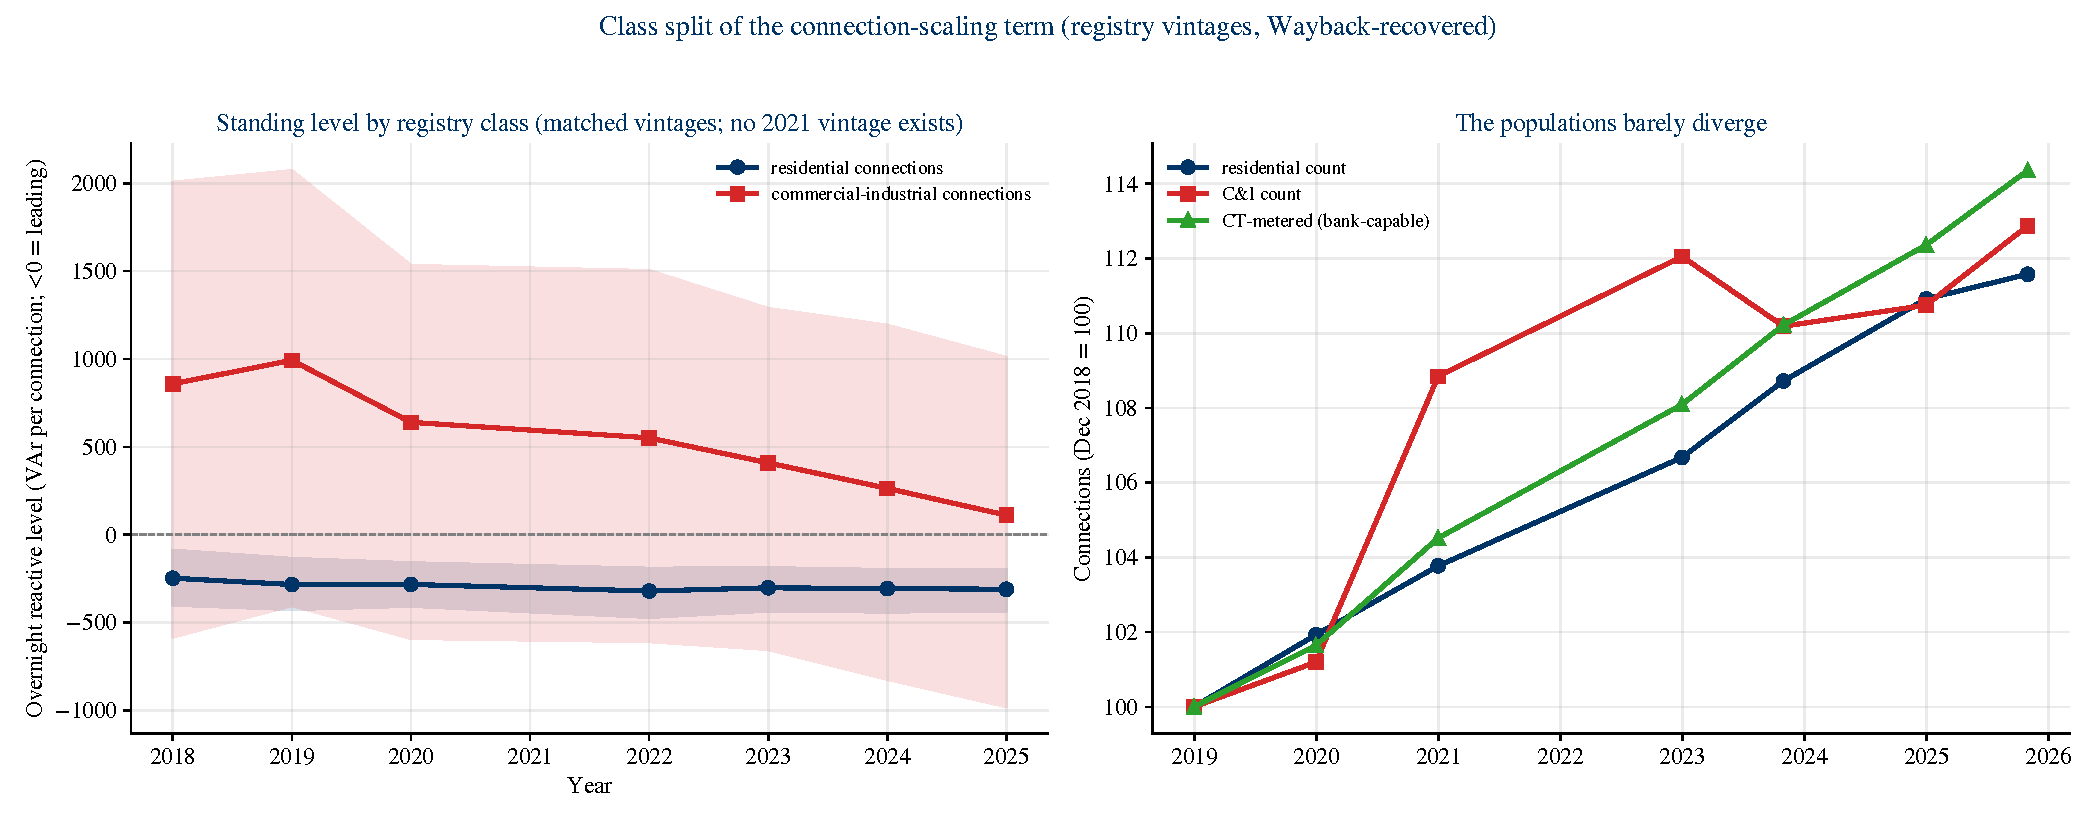
\includegraphics[width=0.92\textwidth]{07_class_split.pdf}
\caption{The connection-scaling term split by registry consumer class.
(A)~The standing overnight reactive level per connection, refitted each year
on that year's own registry vintage: the residential coefficient is leading
and deepening in every year, its interval clear of zero; the
commercial-industrial coefficient descends from net lagging toward zero and
has not crossed it, its interval spanning zero throughout. No 2021 vintage
exists; bands are bootstrap 95\% intervals resampling units. (B)~The class
populations, indexed to December 2018, with the current-transformer-metered
(bank-capable) population: near-parallel growth, no commercial tilt in the
mix. Registry vintages December 2018--July 2026; superseded vintages
recovered from the Internet Archive.}
\label{fig:classsplit}
\end{figure*}

The standing level completes the picture (Fig.~\ref{fig:classsplit}).
Refitted each year on matched vintages, the residential level runs from
$-247$~VAr per connection in 2018 to $-310$ in 2025, leading in every year
with the interval clear of zero. That level, and not the twelve-year change, is
the quantity the bottom-up estimate of Section~V-B predicts, and it lands
\emph{above} the 100--200~VAr per-household band rather than inside it. It should:
the level carries each connection's share of medium-voltage cable as well as its
devices, and Section~IV-C's charging physics puts that share at roughly 190~VAr
per connection nationally (454~MVAr computed for 2025 over 2.34~million
connections), which is the order of the gap. The arithmetic is a consistency
check between two independent computations in this paper, not a decomposition:
it allocates nothing, and the residual inductive limb of Section~V-A sits inside
it. Meanwhile the commercial-industrial level runs from
about $+858$~VAr per connection---net \emph{lagging}---down to $+111$ by
2025, its interval spanning zero throughout. As a class, commercial and
industrial connections still absorb more overnight than they inject; the
margin has fallen by roughly three quarters since 2018, but the crossing the
residential class made years ago has not yet happened there. That standing
position is itself evidence against the stranded-correction reading of the
class's fast per-connection change: a population whose overnight signature is
still net lagging is not one dominated by capacitors left in service, and
part of its change is the overnight motor and process load leaving---the
same departure of the inductive fleet the record shows economy-wide, one
class up. One registry artefact travels with the series: a reclassification
batch of roughly fifteen thousand connections moved into the
commercial-industrial class between the February and March 2020 vintages,
visible in Fig.~\ref{fig:classsplit}(B); it sits inside the class series
without changing the direction of either.

The scaling is also not site size in disguise. Load and connections rise together across sites, so a load-proportional metering
error---the $P\sin\beta$ class of Appendix~A---would mimic connection scaling;
but that class is bounded far below the measured deepening, would concentrate
the deepening in the loaded window rather than equally in both (Section~V-A),
and would over-predict precisely the industrial-weighted sites that in fact fall
short of the fitted deepening.

One rival survives in principle: a load-independent metering-registration drift phased in with meter
replacement. It has no mechanism to produce the connection-scaling term that
carries the deepening, and the connection-independent residual it could sit in
is indistinguishable from zero under every inference scheme, so it is heavily
disfavoured as an account of
the trend while remaining formally excludable only by a measurement that bypasses
the grid-exit metering chain. That measurement is identified and simple---night-time reactive
flow at a residential distribution transformer with a known house count, where
metering on the low-voltage side sees no transformer magnetising and no material
cable charging, isolating the device fleet and splitting the coefficient---and
is the stated next step.

% ======================================================================
\section{From Leading Reactive Power to Overvoltage}
% ======================================================================
\subsection{Why leading reactive power raises voltage}
The relationship to hold in view is that the voltage change along a line depends
mostly on the reactive power and the reactance, $\Delta V \approx (RP+XQ)/V$, with
the $XQ$ term dominant on the grid. When reactive power is lagging ($Q>0$, the
historical norm) voltage drops toward the load, and networks were designed around
this with tap-changers and capacitors to prop voltage up. When reactive power is
leading ($Q<0$, the new overnight reality) the sign flips and voltage is pushed up.
Light load is the dangerous condition because demand is lowest---so little load
absorbs the reactive power or pulls voltage back---while the cable charging is always on. The
mechanism can run away: charging rises with the square of voltage, so a higher
voltage injects more leading reactive power and raises voltage further, and a
protection trip that disconnects a transformer or load leaves the remaining
network carrying more charging per unit of load, stressing the next element in
turn. Two distinct feedback loops run through that description, usually
described as one (Fig.~\ref{fig:loops}). In the first, the \emph{demand-side} loop, disconnected load
takes with it whatever reactive absorption it was providing, and voltage rises;
whether shedding load raises voltage or lowers it therefore turns on the power
factor of what comes off, since lagging load removes absorption while
sufficiently leading load removes a reactive source instead. In the second, the
\emph{plant-side} loop, rising voltage disconnects plant and generation that
were absorbing, and voltage rises further; that loop runs on the response of
protection to voltage and would run the same way behind a demand of any power
factor. In isolated and autonomous systems the feedback is well
documented~\cite{vournas2021,psarros2022}; in neither 2025 blackout did
the lost absorption leave with the demand (Section~VI-C).

\begin{figure*}[!t]
\centering
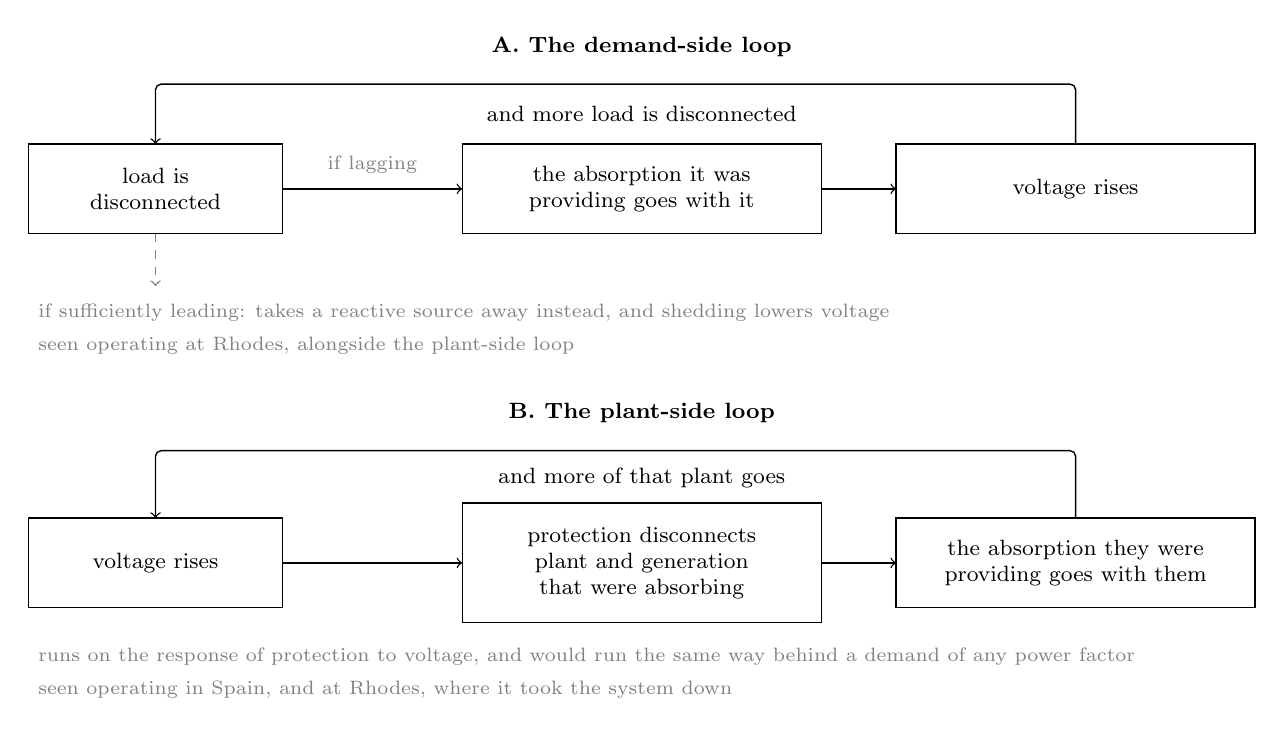
\begin{tikzpicture}[x=0.95mm, y=0.95mm, line width=0.5pt, font=\footnotesize]
% Panel A -- the demand-side loop. Station wording tracks the Section VI-A prose.
\node[font=\footnotesize\bfseries] at (82,81) {A. The demand-side loop};
\draw[->, rounded corners=2] (140,68) -- (140,76) -- (17,76) -- (17,68);
\node at (82,72) {and more load is disconnected};
\draw (0,56) rectangle (34,68);
\node[align=center] at (17,62) {load is\\disconnected};
\draw (58,56) rectangle (106,68);
\node[align=center] at (82,62) {the absorption it was\\providing goes with it};
\draw (116,56) rectangle (164,68);
\node[align=center] at (140,62) {voltage rises};
\draw[->] (34,62) -- (58,62);
\node[gray, font=\scriptsize] at (46,65.2) {if lagging};
\draw[->] (106,62) -- (116,62);
% the sign condition: sufficiently leading load leaves the loop instead
\draw[->, dashed, gray] (17,56) -- (17,49);
\node[gray, font=\scriptsize, anchor=west] at (0,45.5) {if sufficiently leading: takes a reactive source away instead, and shedding lowers voltage};
\node[gray, font=\scriptsize, anchor=west] at (0,41) {seen operating at Rhodes, alongside the plant-side loop};
% Panel B -- the plant-side loop
\node[font=\footnotesize\bfseries] at (82,32) {B. The plant-side loop};
\draw[->, rounded corners=2] (140,18) -- (140,27) -- (17,27) -- (17,18);
\node at (82,23.4) {and more of that plant goes};
\draw (0,6) rectangle (34,18);
\node[align=center] at (17,12) {voltage rises};
\draw (58,4) rectangle (106,20);
\node[align=center] at (82,12) {protection disconnects\\plant and generation\\that were absorbing};
\draw (116,6) rectangle (164,18);
\node[align=center] at (140,12) {the absorption they were\\providing goes with them};
\draw[->] (34,12) -- (58,12);
\draw[->] (106,12) -- (116,12);
\node[gray, font=\scriptsize, anchor=west] at (0,-0.5) {runs on the response of protection to voltage, and would run the same way behind a demand of any power factor};
\node[gray, font=\scriptsize, anchor=west] at (0,-5) {seen operating in Spain, and at Rhodes, where it took the system down};
\end{tikzpicture}
\caption{The two feedback loops. In the demand-side loop, disconnected load
takes the absorption it was providing with it and voltage rises; whether
shedding load raises voltage or lowers it turns on the power factor of what
comes off, which is the quantity Section~III measures moving. In the
plant-side loop, rising voltage disconnects plant and generation that were
absorbing, and voltage rises further; that loop runs on the response of
protection to voltage and would run the same way behind a demand of any power
factor. Spain ran on the plant-side loop. Rhodes ran on both, the plant-side
loop taking the system down and the demand-side loop making the voltage worse
on the way. In North Macedonia there was no compensation plant to lose and no
load was shed at all---the demand-side loop never operated
(Section~VI-C).}
\label{fig:loops}
\end{figure*}

\subsection{The system is already responding}
The New Zealand system is visibly responding to overvoltage pressure from both
ends.

\emph{Distribution capacitors are coming out.} If networks were suffering low
voltage they would be adding capacitors, which raise voltage; instead they are
removing them. From the Commerce Commission disclosures, the
national capacitor-bank count fell from 298 in 2015 to 254 in 2025, and the largest
network removed 47 of 104 banks over the same period. The series is counts only and
shows direction, not MVAr, but the direction is the point: a static-to-shrinking
capacitor fleet cannot be causing a rising leading trend, and the removals are the
signature of the opposite, high-voltage problem. One confound the count cannot see
should be named: the quantity that would matter is not the stock but the operating
practice---banks once switched out overnight and now left in, or the reverse---and
a switching schedule maps one-for-one onto the residual while leaving the count
untouched. No public series records it. The constraint on it is the connection-side
evidence of Section~V-C rather than this count: the population able to hold a bank
accounts for 1.7\% of recent connection growth, the residential class that holds
none carries its own coefficient, and the commercial-industrial class remains net
lagging overnight in every registry vintage.

\emph{Transmission reactors are going in.} Shunt reactors absorb leading reactive
power, and the grid operator has been installing them in the Upper North Island
(Table~\ref{tab:reactors}). Its System Security Forecast records both the practice
and the remedy: ``[o]vernight high voltages are currently managed by removing
selected transmission circuits from service,'' and the two 100~Mvar Pakuranga
reactors ``will dramatically reduce the number of circuit switching operations
required to manage high voltages under N-1 conditions''~\cite{transpower_ssf2022}.
The operator's follow-up study confirms the outcome: with the Pakuranga reactors
and the Hamilton STATCOM in service, ``significant over-voltage issues have not
been observed for current and future light load conditions''~\cite{transpower_ssf2024n1}.
The investments, and the operator's own description of them, are consistent with
managing an overnight overvoltage condition. (A further dynamic device, a
Henderson STATCOM, is proposed under the WUNI Stage~2 major capex proposal but
not yet approved.)

\begin{table}[!t]
\caption{Upper North Island Shunt Reactive Compensation, In Service (Ratings from
Transpower's Interconnection Asset Capacity Disclosures and Project Records)}
\label{tab:reactors}
\centering
\renewcommand{\arraystretch}{1.18}
\begin{tabular}{@{}p{0.40\columnwidth}p{0.22\columnwidth}p{0.22\columnwidth}@{}}
\toprule
\textbf{Asset} & \textbf{Rating} & \textbf{Status} \\
\midrule
Otahuhu reactor R472          & 50~MVAr            & 2022 \\
Pakuranga reactors R562, R582 & 100~MVAr each & 2023 \\
Wairau Road reactor R182      & 63.7~MVAr & in service \\
Hamilton, Otahuhu STATCOMs    & dynamic            & 2023--2025 \\
\bottomrule
\end{tabular}
\end{table}

\emph{And the operator has named the demand-side term.} Transpower's 2023
transmission planning report records that keeping lower North Island voltages
within limits at light load ``requires high levels of reactive power
absorption from the Haywards synchronous condensers,'' and that ``HVDC
transfer may also be limited for harmonic performance if the number of filters
must be reduced to prevent high voltages''; it expects the high-voltage issue
to worsen, and lists ``load characteristics becoming generally more
capacitive'' among the factors~\cite{transpower_tpr2023}. That is the asset
owner, in a planning document, attributing part of the standing pressure to
the electrical character of the load---the quantity this paper measures.

\subsection{The realised risk, abroad}
The regime is not hypothetical. The Iberian event of 28 April 2025 was found to be
a voltage and reactive collapse: the Final Report identifies ``non-effectiveness
of voltage control'' as a root cause; we read it as placing the system's
inability to manage a capacitive excess at the centre of the failure, and it
does not attribute the event to insufficient
inertia~\cite{entsoe_iberia}. The absorption the cascade removed left with the
generation: generators tripped on overvoltage protection, each disconnection
taking its reactive absorption with it, and the under-frequency load shedding
acted only after the generation trips had run their course---the Final Report
finds the scheme delayed the collapse rather than hastening it, while noting it
was not designed for a system in widespread
overvoltage~\cite{entsoe_iberia}. The North Macedonia event
of 18 May 2025 was a cascade of transformer trips from sustained overnight
overvoltage, driven by the high capacitive reactive power of light-load
transmission and distribution networks, with the running wind plant injecting
rather than absorbing and no compensation plant on the system at all---so the
cascade needs neither solar nor distributed generation---and with no load shed:
the demand went only at the end, when the last 400/110~kV transformer tripped,
so the cascade ran with the demand-side loop never
operating~\cite{entsoe_nm}. Each event had local specifics; we read them as
corroboration that the leading-reactive regime is a realised blackout
mechanism, with New Zealand's distinctive contribution the 29-year measurement
and decomposition of how a system drifts into that regime in the first place.

\subsection{Coverage of existing reactive-power provisions}
New Zealand's reactive-power rules were written for the old problem of lagging load
pulling voltage down at the daytime peak. The connection minimum power factor is a
term of the default transmission agreement that binds the distributor for the
aggregate power factor at the connection point---the right party, at the boundary
where Section~III takes its readings---but it applies during regional peak demand
periods and at no other time, the periods themselves fixed by reference to a
transmission pricing methodology replaced in 2023~\cite{eipc_sch126}, so the one
window where overvoltage now lives is the window the rule does not cover; the
reactive-demand measurement provision operates only on weekday hours,
07:00--21:00~\cite{eipc_part8}; and where lines companies charge for power factor,
the published schedules charge on a lagging basis (e.g.,~\cite{powerco_pricing_fy26}). We are careful about
what this does and does not mean. The rules did not \emph{cause} the leading surplus:
Sections~IV and V show the driver is the product-standard demand fleet, outside the
rules' reach, and Section~VI-B shows the capacitor fleet is shrinking, not the legacy of an
over-correcting rule. What the existing provisions do is not cover, price, or limit
the leading reactive power now accumulating overnight. Whether that coverage should
change is a policy question outside this paper's descriptive scope; the descriptive
finding is the measurement, and we note the policy question without arguing it.

One rule moved as the record closed: on 13 November 2025 the statutory
low-voltage supply band was widened from $230~\mathrm{V}\pm6\%$ to
$\pm10\%$~\cite{esr_reg28}. Because each data year here is a whole calendar
year, about seven weeks of the 2025 endpoint sit after commencement rather than
before it. The exposure is small, confined to the last weeks of a twenty-nine
year record, and runs with the reported drift rather than against it; but the
measurement is not strictly pre-commencement and we do not claim it as such.
The widening bears mechanically on what follows. Standing capacitance draws
$Q=\omega CV^2$, so the same fleet delivers about 2\% more reactive power for
each 1\% of sustained voltage elevation the wider band accommodates: some 8\%
more at the new ceiling than was possible at the old one, and about a fifth
more than at nominal voltage. A band that previously forced intervention as
light-load voltages rose no longer does. Post-2025 updates of the
per-connection coefficient should therefore either control for measured voltage
or name the confound: to the extent that light-load voltages rise into the new
headroom, part of any further deepening is voltage-induced rather than fleet
growth.

% ======================================================================
\section{Implications for Power-System Analysis}
% ======================================================================
The measured reversal relocates the binding voltage-security question. For the
lagging era's failure mode---voltage collapse under heavy load---power-system
practice holds a mature, layered stack: automatic under-voltage load shedding as
a last resort, tap-changer blocking, PV- and QV-margin analysis, and decades of
operational tooling, all built on load models of an inductive fleet. In the light-load regime---overnight here and in North Macedonia, and the middle of the day on systems where distributed photovoltaics hollow out net transmission demand---the equivalent layers are thinner in three places: the compensation
provision was sized by voltage level for the old direction, the \emph{automatic}
last-resort layer acts on voltage falling, not rising, and the margin tooling
reports distance to collapse, not to the upper limit. We take those three in
turn, add the load-model correction the measurement makes concrete, and close
with its honest boundary.

The first is a question of what was installed, not of what drives the surplus. The surplus is made at the mains and appears at every level above it, but what stands against it was installed for the old direction. The extra-high-voltage network already carries the switchable reactor fleet its own line charging obliges, and that plant absorbs a demand-side surplus arriving from below as readily as it absorbs its own. The levels between were built for the opposite problem---lagging load pulling voltage down at the daytime peak---and what stands there is capacitor banks. The exposure is thinnest there, and that is where a search should start. It is not a claim that the extra-high-voltage network is covered: both 2025 events occurred there, driven by the network term that dominates at that voltage.

The second is the standard emergency lever, built for the falling direction; in
this regime its effect on voltage is no longer of one sign. In a collapse, shedding
load is corrective: every megawatt shed relieves the stress that is depressing
voltage. In the light-load capacitive regime the two loops of Section~VI-A
separate. What shedding does to voltage in the demand-side loop turns on the
power factor of what comes off---lagging load takes absorption away with it;
sufficiently leading load takes a reactive source away instead---and that
power factor is the quantity Section~III measures moving through zero, so a
scheme designed on the lagging assumption can no longer assume it. The
plant-side loop is indifferent to what the demand draws---protection that
removes absorbing plant raises voltage behind a demand of any power
factor---and it is the loop the Iberian cascade ran on; in North Macedonia
the demand-side loop never operated at all (Section~VI-C).

In the Iberian event the voltage kept rising as the under-frequency stages acted, for
reasons the Final Report locates in the network and the generation rather than
in the shed demand: the shedding reduced line currents, leaving higher
residual voltage and more line charging, while the simultaneous disconnection
of generators reduced voltage control and absorption~\cite{entsoe_iberia}. The
Rhodes cascade of 2016 is the one investigated event in which the demand-side
loop can be seen operating: under-frequency shedding raised voltage and
deepened generator reactive absorption---an aggravator in a collapse
ultimately triggered on loss-of-field, and one a small shunt reactor would
have prevented~\cite{vournas2021}---and rerunning the disturbance with fewer
shedding stages avoids the overvoltage while holding the same frequency nadir.
No investigated event attributes a blackout to the demand-side loop. And on
the demand character measured here the implication runs further: net-leading
demand takes a reactive source with it when it trips, so the classic
load-rejection voltage rise weakens and can reverse in sign, and the
overvoltage exposure in an event concentrates on the plant side---the
absorbing plant and generation that protection removes, and the under-excited
operating points where the autonomous-system record already places the
failure path and its countermeasures (under-excitation limiters blocked for
isolated generators feeding capacitive networks; any voltage-setpoint change
made in the absorbing direction)~\cite{vournas2021}. The
last-resort schemes discussed here were all designed for the other direction:
none connects load or absorption when voltage runs away, and none reads the
power factor of what it sheds.

Two things about the surplus bear on that second leg. The distinction between
the drift and the level matters here (Section~IV): the \emph{drift} into
the regime is dominantly the demand fleet, but the standing light-load surplus the mechanism feeds on is substantially long-standing distribution network charging that the fleet's shift has uncovered---distributed, always energised, scaling with the
square of voltage (Section~VI-A), and not itself dispatchable, since its removal
means switching circuits out of service, spending N-1 security to buy voltage
margin (Section~VI-B). The cascade arithmetic is then inverted relative to
collapse: each element lost in a voltage collapse---a stalled motor tripping,
load disconnecting---reduces the demand that is depressing voltage, so the
disturbance partly self-relieves, whereas in the plant-side loop each
definite-time protection operation removes absorption and strengthens the
driver, so the disturbance self-reinforces in quantised, irreversible steps---the
arithmetic of both 2025 events (Section~VI-C).
The Iberian sequence ran from first protection operation to blackout in well
under a minute~\cite{entsoe_iberia}; the North Macedonian event shows the same physics grinding through a lightly compensated system over hours~\cite{entsoe_nm}; the autonomous-system literature finds the positive
feedback sharpest in small and weakly interconnected
systems~\cite{vournas2021,psarros2022}.

The third is the margin tooling. Overvoltage protection and locally automatic
shunt switching exist as device-level controls, and the QV curve's upper limb,
temporary-overvoltage studies and self-excitation screening each address part of
the question; but none is reported as a routine margin quantity the way PV and
QV margins report distance to collapse, and the field's 2026 mechanisms review
likewise proposes containment countermeasures for the upper band without
proposing a margin quantity for it~\cite{vournas2026review}.

The analysis stack under-represents the regime it is entering. Planning and
protection studies still commonly represent demand with constant, lagging
power-factor archetypes calibrated to the motor-dominated fleet, and expert
reviews have already documented the error constant-power-factor load modelling
introduces~\cite{cigre_tb719,epri_loadmodel}; the measured net overnight flow
now carries the opposite sign, so the studies most responsible for revealing the
risk are calibrated to a fleet that no longer describes the night. That reaches
past the archetype: by the sign argument above (Section~VI-A), a shedding or load-rejection study calibrated on lagging demand carries an unexamined sign at light load. The gap is calibration rather than structure. The standard composite load model does carry a distribution-side shunt term---but not as an inventory of plant: its value is computed at initialisation ``to balance the reactive consumption of the load devices and of the transformer and feeder with the load Q value specified in the power flow data'', and it is then allocated across the load components in proportion to each one's share of megawatts~\cite{wecc_cmpldw}. The model therefore inherits whatever reactive character the power-flow case carries, and at light load---the condition such cases have least often been built against a measured demand character---it reproduces a lagging archetype as though it were measured plant. Where demand is then lost by tripping whole feeders---under-frequency or interruptible-load schemes---the capacitance behind them is genuinely de-energised with them, so removing it is correct in direction, and the megawatt weighting is second-order: a large representative block sheds connections and megawatts in similar proportion. Only where a device stops drawing while its supply stays live---the specification's end-use protection case, in which the allocated capacitance is ``tripped in proportion to the MW of each component tripped''---does the removal run against the physics. The sequence matters as much as the mechanism. Under-frequency and interruptible-load schemes act on frequency, so in a voltage-led disturbance they operate only once enough plant has been lost to move it: of the three investigated events, one shed no load at all and in another the absorption left with the generation (Section~VI-C), while in the third shedding aggravated a collapse already running on loss of field (Rhodes, above). What the demand contributes at initiation is therefore a standing level rather than a trip---and the standing level is the part the initialisation inherits rather than measures.

The measurement gives the load-model correction a concrete, portable form. The
light-load fleet needs a net standing shunt term that scales with
connections served---on the New Zealand panel, about 210~VAr per connection
accumulated over 2013--2025 (Section~V-C; a boundary-level figure that carries
each connection's share of network cable with it)---alongside
whatever power-factor archetype represents the operating draw. A
constant-power-factor archetype cannot represent this term even qualitatively:
it is present when the load is not drawing; it accumulates behind
existing connections rather than arriving with demand growth---the coefficient
of Section~V-C is fitted per connection and refitted each year, so a fleet
growing only in step with new connections would leave it flat, whereas it swept
some 300~VAr per connection across the record---so it will not surface in load
forecasts either; and it is young and moving---on the inductive side of zero
early in the 2010s, accumulating faster over the second half of the window than
the first (Section~V-C)---so archetypes calibrated even a decade ago predate
the term entirely.

None of this makes the regime unmanageable. With fast absorption installed, New
Zealand's operator reports no significant overvoltage issues under current and
future light-load conditions (Section~VI-B): what is missing is not feasibility
but architecture---the compensation provision, the automatic defences, the
security-margin tooling and the load models were all built for the direction the
system has left. Their redesign is
development work beyond this paper's descriptive scope. What the measurement
supplies is the direction and the rate: a national boundary flow that has
crossed to the capacitive side of the axis around which those tools were built,
driven dominantly by the load fleet, at about $-0.018$~MVAr per MW of overnight
load per year, with the crossing already behind it.

% ======================================================================
\section{Future Work}
% ======================================================================
The measurement opens more questions than it settles. We collect here the ones
it makes tractable, several of which consolidate pointers made throughout.

\emph{The attribution measurement.} The first priority is the decisive test
named in Section~V-C: night-time reactive flow at a residential distribution
transformer with a known house count, which isolates the device fleet from the
per-connection cable share, complemented by bench measurement of the standing
injection of common device classes in standby. One instrumented night and one
instrumented bench would move the central hypothesis of Section~V-B from
labelled to tested.

\emph{How long can it run?} The coefficient's history (Fig.~\ref{fig:icp}B)
shows acceleration, not saturation. A single adoption curve must eventually
saturate, but the fleet is a \emph{succession} of curves---lighting, broadband
equipment, heat pumps, and next an electric-vehicle charging and home-battery
fleet expected to carry the largest input filters yet---so extrapolation calls for a
renewal model of device generations---each wave layered on and later
replaced---rather than a logistic (single saturating S-curve) fit to the total.
Bounding scenarios (the present $\sim$20~VAr per connection per year held
constant; saturation at the current device census; the vehicle wave layered
on top) built from appliance-stock and sales data would bracket the 2030s
trajectory. Nothing in the record yet marks the turn.

\emph{Whether any instrument should see it.} The standing term currently
falls outside every instrument that could notice it: asset registers, load
models, demand forecasts, product standards (Section~I-A), and reactive-power
provisions written for lagging daytime load (Section~VI-D). Whether any of
them should see it---and at which level: product standard, connection
requirement, or network tariff---is a question of standards development and
regulatory economics beyond this paper's descriptive scope. We note only that
the relative economics of absorbing the surplus at the grid level against not
creating it at the product level appear to be unquantified in the open
literature, and that the quantity now accumulates at a measured, forecastable
per-connection rate.

\emph{Power-system analysis.} Four concrete developments follow from
Sections~V and VII: a connection-indexed net standing shunt term and its
placement within composite load-model structures; a routine margin quantity
for the upper voltage band---distance to capacitive runaway---analogous to the
PV and QV margins of the collapse toolkit; the frequency-domain counterpart,
since distributed shunt capacitance reshapes the network's harmonic impedance
as well as its fundamental-frequency balance---if the term accumulates behind
every connection, the parallel resonance a network presents to the transmission
system falls year on year toward the low-order harmonics, which is a screening
quantity the same measurement supplies and no part of this paper's fundamental
frequency analysis addresses; and the automatic last-resort
defence architecture for the overvoltage direction, whose absence Section~VII
records (the 2026 review proposes transmission-level elements of one---tap-changer
blocking on instability detection and emergency converter reactive absorption
above 1.08--1.10~pu~\cite{vournas2026review,vournas2026epsr}---leaving the
demand-side term itself unaddressed).

\emph{Replication and the meter fleet as instrument.} The test needs only
settlement metering and connection counts, so any operator can reproduce it;
comparative axes of interest include heating-electrified against
gas-heated building stocks; systems whose device adoption leads New
Zealand's, such as Norway's vehicle fleet; and the mains-voltage axis itself,
since if the filter is the mechanism the per-connection drift should order as
$\omega V^2$ from Japan through North America to the 230-volt world
(Section~V-B). And where advanced meters record
reactive energy at the connection itself, the per-connection term could in
principle be read directly and continuously from the metering fleet, closing
the chain from device to grid without new instrumentation.

\emph{Separating the two limbs.} Section~V-A establishes that the measurement
returns $Q_L-Q_C$ and never either limb. Two routes could split it, and neither
needs new field instrumentation. The first anchors the inductive limb at the start
of the record: the national household end-use project metered real and reactive
power in nine houses over 2002--2004 and found the always-on standing load at
0.5--0.7 power factor inductive~\cite{heep_sr155}; if its standing real power per
house is recoverable, $Q_L = P\tan\phi$ converts that directly into a starting
level in VAr per household, against which the level history of
Fig.~\ref{fig:icp}B could be read as a retreat. Its caveats (Section~V-C) apply:
nine non-randomly selected houses, and a total rather than a displacement power
factor. The second is frequency sensitivity, which returns the \emph{sum} where
the level returns the difference: $Q_C=\omega C V^2$ rises with frequency while
$Q_L=V^2/\omega L$ falls, so at fixed $P$, $\mathrm{d}Q/\mathrm{d}f =
-(Q_L+Q_C)/f$, and two equations resolve two unknowns. Feasibility is the open
question and should be scoped before the method is relied on: half-hourly
averaging smears frequency excursions to perhaps $\pm0.05$~Hz of usable variation,
the load's own frequency response in $P$ and $Q$ confounds it, and what it returns
is the total system $L$ and $C$ including cable charging and transformer
magnetising, from which Section~IV-C's computed cable term would have to be
subtracted.

\emph{A fitted circuit model.} A companion study, in preparation, fits the
circuit form directly: a standing term with drift and dated operational
steps, load-composition and series terms, and embedded-plant signatures,
fitted at every grid exit point and validated element by element against
dated network events, connection counts, and metered embedded generation.

% ======================================================================
\section{Conclusion}
% ======================================================================
Using 29 years of regulatory half-hourly metering, we measured a national power
system's reactive character shifting from lagging to leading at supply-point
resolution: on the balanced demand panel (the same 123 grid exit points
throughout), mean overnight
reactive power fell from about $+466$~MVAr to about $-451$~MVAr (about
$-31$~MVAr/yr), crossing net-leading overnight in 2016 and at the
evening peak only later---a measured phenomenon, not a metering artefact,
holding in winter and summer alike, within the modern metering-fleet era alone,
and with every contaminated grid exit point removed. The drift is dominantly
the demand side: a first-principles charging calculation that fits no cable
coefficient puts the organic share at about 80\% (physical band 75--88\%) over
the 2013--2025 asset-disclosure window, with the two statistical methods
corroborating the direction over the full record but not pinning the split.
And the connection-scaling test identifies what the demand side is physically
doing: at about 210~VAr per connection added over 2013--2025, with no detectable
connection-independent residual, from a term that sat on the inductive side of
zero into the 2010s and has accumulated faster over the second half of the
window than the first, the load fleet is not merely drawing fewer lagging vars
overnight; its own standing shunt term is moving capacitive.

The defences,
margins, and load models of power-system practice were built for lagging load and
the undervoltage direction; the measured overnight flow has crossed to the other
side, where no last-resort scheme is addressed to voltage rising and, in the
plant-side loop, each protection operation reinforces the disturbance
(Section~VII); the same regime
has produced two realised blackouts abroad, and the New Zealand system is
already responding to it from both ends while its deeper demand-side driver
remains unnamed in the rules. New Zealand's record---an advanced-state, small,
isolated, heavily cabled analogue whose net-leading crossing preceded the 2025
European events by nearly a decade---is, to our knowledge, the longest direct
measurement of that crossing. If the standing term is carried by the
globally standardised product fleet, every system connected to the same supply
chain is accumulating it on a similar schedule, at a dose set by its supply
voltage (Section~V-B)---on 230-volt systems roughly three times the
North-American rate per device and four to five times the Japanese, so the
dose ordering maps the exposure geographically and is itself the decisive
comparative test, an ordering that places the lower-voltage fleets
structurally later on the same accumulation, not exempt from it. Supply
voltage sets the dose; transmission voltage sets its visibility. The term is
created at the mains, indifferent to the network above it, while in any system-wide reactive account the boundary flow that would reveal it is dwarfed by the transmission network's own charging, which grows with the square of transmission voltage and with route length---so New Zealand's 220-kV maximum is an unusually transparent window, and in a 400-kV system that contrast is several times sharper
(against 220~kV the voltage terms alone give $(400/220)^2\approx3.3$, and
route length---which extra-high-voltage networks exist to span---widens it),
where a network-side reading of the surplus is the natural one (the reading
both 2025 investigations took, Section~I-C). The claim is therefore priority
of measurement, not of exposure: the failures arrived first where the network
term is largest, not where the demand-side term is clearest. The systems with
the most to gain from such a record
are the ones without one: larger fleets, no measurement of the demand-side
term, and, in Europe's case, a demonstrated failure mode.

The record also says where this goes. The drift shows no sign of slowing: the
per-connection coefficient accumulated faster over the second half of the
window than the first, was running at about 20~VAr per connection per year at
the 2025 end, and the next device waves---an electric-vehicle charging and
home-battery fleet expected to carry the largest input filters yet---are
still arriving; nothing in the record yet marks the turn. Tracking that
coefficient with a renewal model of device generations, and the decisive
attribution measurement at a residential distribution transformer
(Section~V-C), are the nearest work (both detailed in Section~VIII).

The stability question has moved with the sign: with overnight demand now
net leading, defence design points at plant-side absorption---ride-through of
absorbing plant, coordination of under-excitation limits on generators
feeding capacitive networks~\cite{vournas2021}---and at solved network cases
of the light-load state, which this boundary record cannot settle; and
because the same $V^2$ scaling sets a network's own charging per kilometre,
systems pairing extra-high-voltage networks with 230-volt fleets---Iberia's
400~kV among them---carry both terms at once. The prediction also runs the
other way: unlike the passive filter fleet, the arriving wave of vehicle
chargers, photovoltaic and battery inverters is controllable, and
interconnection standards already define the response modes to steer
it---IEEE Std 1547-2018 carries a voltage--reactive-power (volt-var) mode
among its reactive-power controls and requires Category~B resources to be
capable of absorbing, as well as injecting, reactive power to at least 44\%
of nameplate apparent-power rating~\cite{ieee1547}. Large inverters operated,
or required, to absorb at light load---running in the lagging quadrant
against the fleet they share a board with---are then the natural first
counter to the leading surplus at the grid exit point. Nearer the customer,
the distribution networks the reverse flow transits hold two margins in
records they already keep: tap-changer position histories---how much
regulation headroom remains at light load---and the loss cost of the
standing circulating current.

The limitations are stated throughout: the balanced panel controls churn but does
not eliminate it; the decomposition attributes the drift, not a causal mechanism in
any single load; the exact organic share and the level composition are not
point-identified; the measurement gives the net standing term and not its
inductive and capacitive limbs separately, so the device-level attribution of
the connection-scaling term remains a labelled hypothesis for the capacitive
limb, with its decisive low-voltage measurement identified; and a single national system is one observation---offset, not cured, by its
position as a leading-edge analogue and by the two independent European
corroborations. The defence-scheme and load-model development this measurement
motivates is separate work. What this paper offers is the measured trajectory,
its decomposition, the term it identifies, and the direction power-system
analysis must now build for.

\appendices
\section{The Measurement, Not the Trend}
This appendix carries the measurement-error analysis summarised in
Section~II-C: the bound on the one error that does not average down, the timing
argument for the 2010--2013 fleet replacement, and the test for a synchronous
system-wide re-base.

\subsection{The measurement chain, and what is documented of it}
The quantity at risk is not the meter's arithmetic but the phase relationship
presented to it. A grid-exit-point metering installation is a chain: current
and voltage transformers on each phase, their secondary wiring and burden, and
the meter. The meter end of that chain is well documented and tightly held---
Class~0.2S for active energy, a certified Category-5 installation on a
36-month re-certification and 19-month inspection cycle---and the reactive
class, though looser, is at least stated. The transformer end is neither.

The Code specifies the meter classes directly but takes the instrument
transformers to their own standards: Schedule~10.1's table of standards for
metering components lists the IEC~60044 series for current, inductive voltage,
combined, capacitor-divider and electronic transformers, since superseded
internationally by IEC~61869~\cite{eipc_part10}. It imposes no accuracy class
of its own on them. Its one phase-displacement parameter, in the polyphase
table, limits how far the phases of an installation may differ \emph{from each
other} (2$^\circ$, irrespective of power factor); it says nothing about a
displacement the phases share, which is precisely the component that survives
averaging. Below that, three things are simply not in the public record:
the class, ratio, burden and vintage of the transformers at any individual
site; whether the overnight current at these points falls below the range over
which the classes specify anything; and whether the 2010--2013 programme
touched the transformers at all---the asset management plan that dates it
records the replacement of the revenue \emph{meters}~\cite{transpower_amp}.

Nor do the classes bind tightly where this paper looks. The IEC current-transformer
classes specify accuracy only down to 5\% of rated current---1\% for the
extended S classes---and permit three to four times the rated-current error at
that bottom point~\cite{ccs_an136}; the reactive meter class is specified only
above 20\% of rated current and gives no bound below it~\cite{eipc_part10}. A
metering chain at overnight minimum is therefore operating where its own
specifications thin out, and the effect of a given phase displacement on the
reactive reading is largest exactly there, since the overnight aggregate power
factor sits near unity and the reactive component is small. This is why the
term is bounded by assumption below, with the assumption made explicit and
varied, rather than read off a documented class.

\subsection{The bound on the phase-angle bias}
Section~II-C states the random-error case in full: class-bounded, bidirectional
across 123 points and 29 years, it averages down and needs no more here. The
systematic case deserves the full bound. A phase displacement $\beta$ anywhere
in the chain rotates the measured current phasor and injects a spurious
reactive term of approximately $P\sin\beta$: proportional to the metered load,
independent of the reactive power being measured, and concentrated in exactly
the window this paper measures.

The limits above bind each chain independently, and the panel's 123 supply
points carry several hundred separately specified transformer sets on their
several hundred phases. Displacements enter with either sign and average down
with the rest of the random budget; what does not average down is the
\emph{common-mode} part, the displacement every set shares. Suppose,
generously, that this were half a degree across the whole panel. The spurious
term is then about 0.9\% of $P$---under 20~MVAr on the $\approx$1,900-MW
overnight panel---a near-static offset roughly fifty times smaller than the
measured 900-MVAr swing, and one that moves the crossing year by about half a
year at most. Because the term scales with $P$, which grew by only about
280~MW over the record, it can contribute only about 0.1~MVAr/yr of apparent
drift against the $-31$~MVAr/yr observed.

The result does not turn on the half degree. At three times it---1.5$^\circ$,
the order the classes themselves allow at the bottom of their specified range,
applied coherently to every set---the offset is still under 50~MVAr, about an
eighteenth of the swing, and the apparent drift about 0.26~MVAr/yr, two orders
of magnitude below the measured rate.

In fact the magnitude does not matter at all, which is the stronger form of the
argument. A \emph{static} common-mode displacement generates apparent drift
only through the growth of the load it multiplies, so the most it can generate
across the record is $\Delta P\sin\beta$, and $\sin\beta \leq 1$. Overnight
panel load grew about 280~MW. Even a physically absurd 90$^\circ$ displacement
on every transformer set therefore falls short of the measured 900-MVAr swing
by a factor of three. No static bias of any size reproduces this trajectory.

The phase-displacement route to the drift consequently requires $\beta$ itself
to move across the record---a drifting bias, not a fixed one---and three things
work against that. Drift within the instruments is worked against by the
re-certification and inspection cycle. A reset at the 2010--2013 meter
replacement would enter as a step, and the series shows none. And the bias
would have to move coherently across sites to survive averaging, which is the
hypothesis the re-base test below examines directly and rejects. The
phase-angle bias can therefore blur the \emph{level} by tens of MVAr; it cannot
manufacture the \emph{drift}. Independently, no instrument error has reason to
be cable-correlated (Section~IV) or to scale with the connections behind each
meter (Section~V-C).

\subsection{The 2010--2013 fleet replacement}
The one metering transition in the record is bounded by its timing. The
staggered 2010--2013 replacement of the legacy PSI~Quad4 instrumentation by
four-quadrant ION8800A meters was an \emph{upgrade} that improved the recording
of leading (export) reactive power. Its possible bias is anchored at both ends
of the record. At the 1997 anchor, leading flows were about 1\% of overnight
half-hours, so any under-recording of leading reactive power by the older fleet
cannot materially bias the $+466$~MVAr starting point; the 2025 anchor sits
wholly on the modern four-quadrant fleet, the instrumentation best able to
measure the leading regime. The endpoint-to-endpoint swing is therefore
insensitive to the upgrade, which could at most distort mid-period
curvature---and in the conservative direction, since under-recorded leading
reactive power would delay, not advance, the measured crossing. The upgrade also
pre-dates the lagging-to-leading crossing (2016 on the demand panel, 2020 on the
full panel), so the leading regime, the novel part of the claim, is observed
wholly on the modern fleet. Directly on the data: the per-MW drift measured
within the modern-fleet era alone (2014--2025) is $-0.019$~MVAr/MW/yr against
$-0.018$ over the full record---if anything steeper---so the trend is not
inherited from the older instrumentation.

\subsection{Test for a system-wide metering re-base}
The two arguments in Section~III-B address gradual or staggered metering change. A
single system-wide change is different: a one-date revision of sign convention or
central processing would step every grid exit point in the same year and the same
direction, a fingerprint no gradual physical trend leaves. We test for it
(Fig.~\ref{fig:splice}). Each grid exit point is first detrended by its own robust
(Theil--Sen) line---robust so that a step, were one present, is not partially
absorbed into a tilted least-squares fit and hidden---and the residuals are
standardised by each site's own scatter; what remains is each site's wobble about
its own path. Two per-year summaries are then taken across sites: the median
residual (the ``common wobble,'' near zero while wobbles are idiosyncratic, jumping
only if sites move together) and the coherence, the share of sites on the same side
of their own trend that year. Local causes cannot coordinate a hundred separate
substations' deviations within a single year, but a central processing change
would: a genuine re-base drives coherence toward 100\%. An off-the-shelf
change-point detector---which is forced to mark steps even on a smoothly bending
curve, so its candidates are hypotheses rather than verdicts---flags years around
2002 and 2022; the earlier candidate abuts
the 2000--2001 metering-vintage step flagged in Section~III-B, and coherence at the
candidates is only 67\% and 69\% against a typical-year 62\%, indicating curve-bends
rather than a coordinated re-base. The highest coherence anywhere, 75\% in 2025, merely reflects most
sites being leading together at the end of the record because the whole system has gone
leading. No synchronous re-base underlies the trend.

\begin{figure*}[!t]
\centering
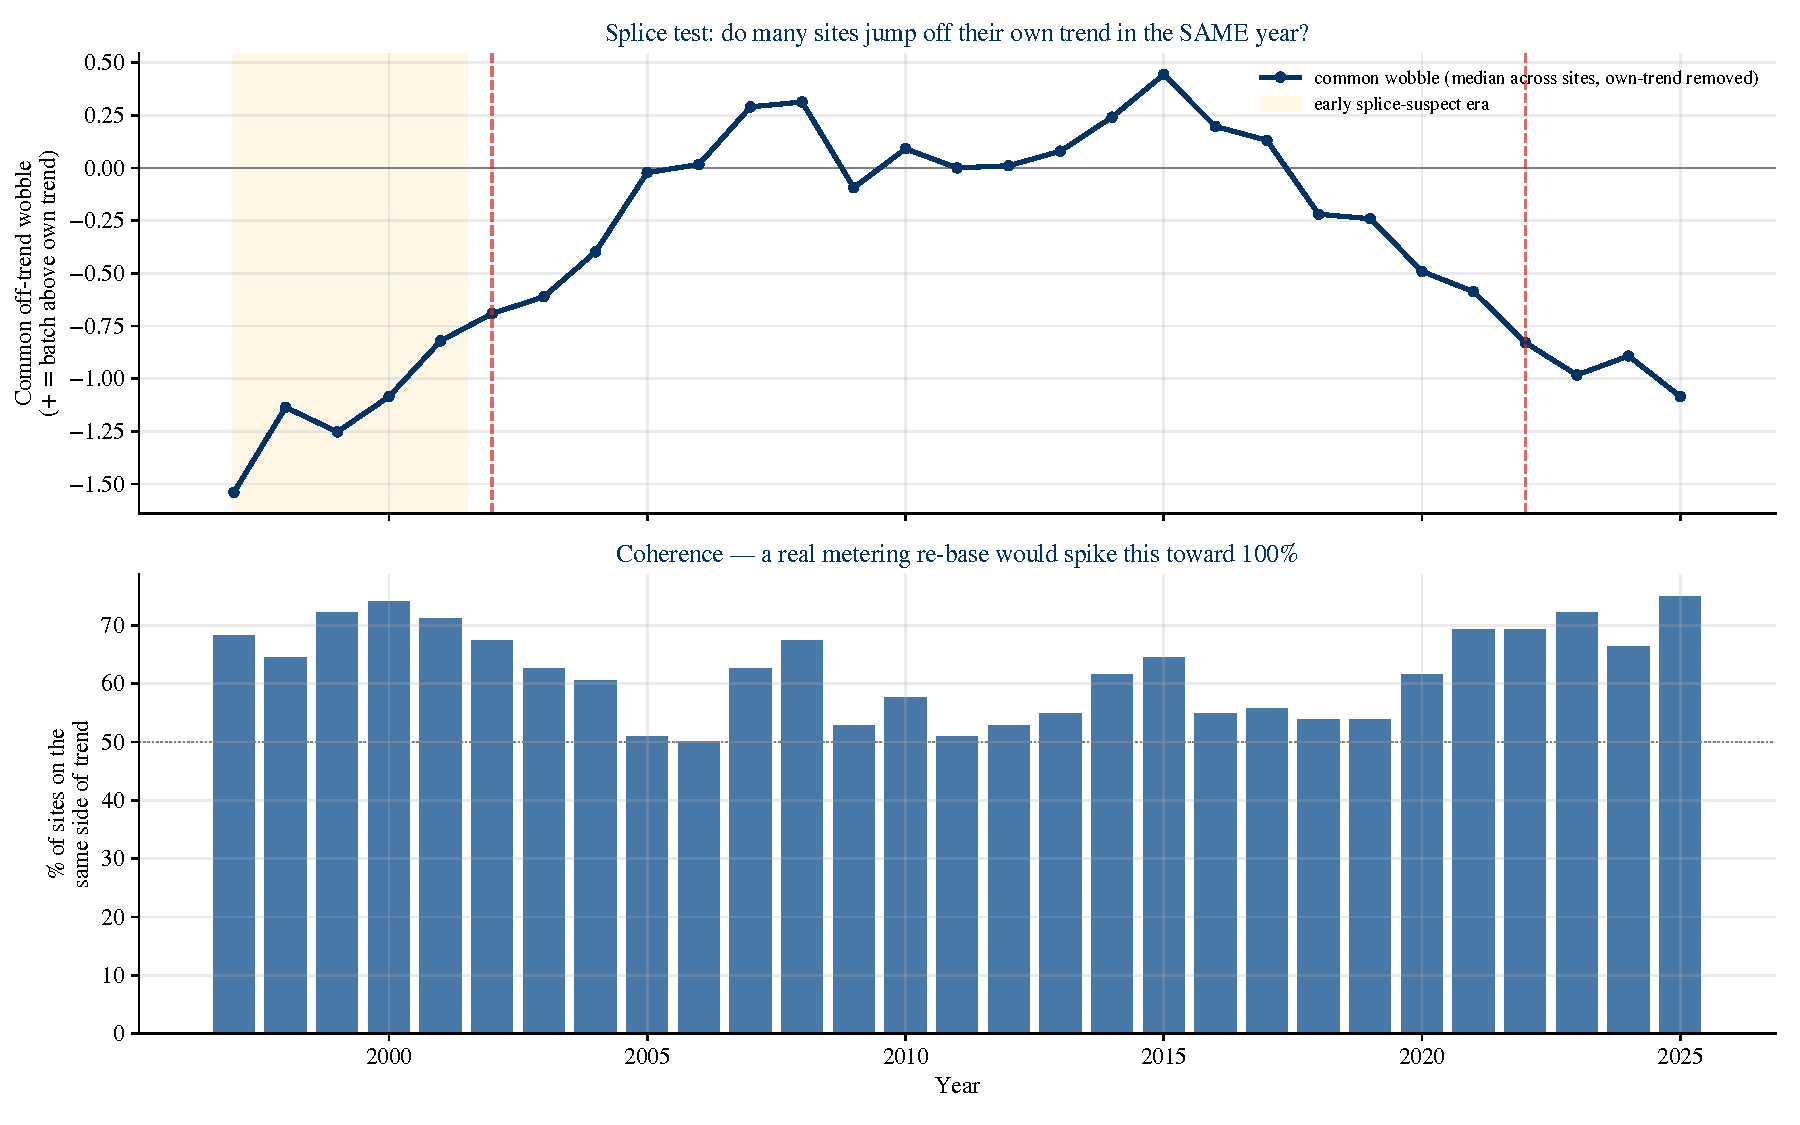
\includegraphics[width=0.57\textwidth]{01_splice_test.pdf}
\caption{Test for a system-wide metering re-base (the ``splice'' of the
in-figure title: the join between metering eras). Each grid exit point is detrended by
its own robust (Theil--Sen) line; the upper panel is the median residual across sites
(the ``common wobble'') and the lower panel the coherence, the share of sites on the
same side of their own trend each year. A genuine re-base would spike coherence toward
100\% in a single year. The change-point candidate years (about 2002 and 2022,
the dashed verticals) reach only 67\% and
69\% against a typical-year 62\%: curve-bends, not a coordinated re-base.}
\label{fig:splice}
\end{figure*}

\section{The Mains Input Filter at 50~Hz}
This appendix carries the component-level basis for the Section~V-B
hypothesis: what the electromagnetic-compatibility (EMC) filter is, why it is
universal, and what it presents to the 50-Hz network.

\subsection{Why the filter exists}
A switched-mode supply chops current at tens to hundreds of kilohertz. Left
unfiltered, that switching noise conducts back through the supply cord into the
mains network. Conducted-emission limits (the international CISPR
limits~\cite{cispr32}, covering roughly 150~kHz--30~MHz) are a condition of
sale in most jurisdictions, New Zealand included, and the universal compliance
solution is a passive low-pass filter at the appliance's own mains terminals.

The mandate's chronology brackets the measured record. The conducted-emission
limit structure dates to CISPR~22:1985, absorbed by CISPR~32 in 2012 and
applied in New Zealand as AS/NZS~CISPR~32; New Zealand law has made compliance
a condition of sale since at least 2001 (supplying non-compliant equipment is
an infringement offence), lists switched-mode power supplies by name at the
test-report conformity level, and---verified by full-text search of the
current notice---contains no harmonic-current or power-factor requirement of
any kind~\cite{rsm_emc2019}. Regulatory force, too, predates the record: the
European Union applied the harmonised EMC requirement from 1 January 1992
(Directive 89/336/EEC~\cite{eu_emc1989}) and permitted apparatus conforming
to prior national regimes only until 31 December 1995 (Directive 92/31/EEC),
so the directive's conformity route has been the sole lawful route to that
market since 1996, carried through recasts to the current Directive
2014/30/EU, applying from 20 April 2016. A mandate that old cannot date the
knee of Fig.~\ref{fig:icp}B: what moved is the population beneath it. A
wire-wound transformer needs no filter---the New Zealand notice leaves it at
the lowest conformity level---so the mandate's standing capacitance arrived
only as the switched-mode classes scaled through the 2000s and 2010s, wave by
wave, on the schedule Section~V-C's coefficient history measures.

On the exit side, external-power-supply no-load
efficiency floors (California 2004; ENERGY STAR December 2004; United States
statute for units manufactured from 1~July 2008, no-load $\le$0.5~W~\cite{eisa2007};
the European Union staged to 0.30~W by April 2011; New Zealand's own mark~III
floor from 9~June 2011~\cite{nz_eps2011}) made the iron-core linear supply
progressively
unsaleable, and the trans-Tasman regulator's own review records that
international standards propagate to the New Zealand market through the global
supply chain on a six-to-eight-year lag~\cite{eeca_eps2025}. Applied to the
rungs, that lag places the New Zealand shelf-stock conversion between about
2010---the earliest rung plus the shortest lag---and about 2019, the last rung
plus the longest: a decade-long window that straddles the crossing of
Fig.~\ref{fig:icp}B rather than dating it. Only the last of these rungs was
ever New Zealand law, which is why the conversion is read off the supply chain
and not off the domestic instrument.

\subsection{The circuit, and what 50~Hz sees}
Fig.~\ref{fig:emifilter} shows the standard arrangement; the safety-class
rationale for why the line-to-neutral \emph{X-capacitors} are the one large
element (metallised film, typically 0.1--2.2~$\mu$F, commonly one each side of
the choke) is carried in Section~V-B. The \emph{common-mode choke}
(two coupled windings on a shared core) presents high impedance to noise
leaving on both conductors together and negligible impedance at 50~Hz;
\emph{Y-capacitors} (line-to-earth and neutral-to-earth) are held to
nanofarads by touch-current limits and are electrically negligible here---where
the appliance is earthed the line-to-earth element does inject at the
fundamental, but at nanofarad scale that is under a per cent of the
X-capacitor beside it, and the numerous small always-connected devices are
double-insulated with no protective earth at all, so counting X alone biases
the estimate very slightly low; a
megohm-scale discharge resistor completes the set. At the fundamental
the only material injection is therefore the X-capacitance, which draws
pure leading current whenever the plug is live: $Q=\omega C V^2$, so at 230~V,
50~Hz, 0.1~$\mu$F injects 1.7~VAr, 0.47~$\mu$F injects 7.8~VAr, 1~$\mu$F
injects 16.6~VAr, and 2.2~$\mu$F injects 36.6~VAr.
Table~\ref{tab:xcapclasses} carries the census behind Section~V-B's
per-device figures---typical total class-X capacitance by device class, and
the standing injection that capacitance draws on this mains and on North
America's, where the same component earns a third of the reactive power. The
two zero rows are as load-bearing as the populated ones: the sub-20-W charger
swarm and the retrofit LED lamp contribute essentially nothing, which is why
the standing term concentrates in the always-connected classes above about
25~W.

\begin{table}[!t]
\caption{Typical Total Line-to-Neutral (Class X) Capacitance by Device Class,
and Its Standing Injection on Two Mains}
\label{tab:xcapclasses}
\centering
\renewcommand{\arraystretch}{1.18}
\begin{tabular}{@{}p{0.40\columnwidth}p{0.15\columnwidth}p{0.15\columnwidth}p{0.15\columnwidth}@{}}
\toprule
\textbf{Device class} & \textbf{X cap.\ ($\mu$F)} & \textbf{VAr, 230~V 50~Hz} & \textbf{VAr, 120~V 60~Hz} \\
\midrule
USB charger $\le$20~W & none found & $\approx$0 & $\approx$0 \\
LED retrofit lamp $\sim$5~W & not fitted & $\approx$0 & $\approx$0 \\
USB-PD and laptop supplies 27--65~W & 0.10--0.22 & 1.7--3.7 & 0.5--1.2 \\
Laptop and retail supplies 65--140~W & 0.22--0.47 & 3.7--7.8 & 1.2--2.6 \\
LED driver 12--100~W & 0.066--0.45 & 1.1--7.5 & 0.4--2.4 \\
TV / monitor supply 100--220~W & 0.44--0.66 & 7.3--11.0 & 2.4--3.6 \\
Desktop computer supply & 0.37--1.8 & 6.1--29.9 & 2.0--9.8 \\
Whiteware (laundry, inverter refrigeration) & 0.47--1.41 & 7.8--23.4 & 2.6--7.7 \\
Heat-pump / AC outdoor unit & 1.41--2.0 & 23.4--33.2 & 7.7--10.9 \\
Single-phase VSD input filter & 0.94--4.2 & 15.6--69.8 & 5.1--22.8 \\
Generic appliance filter, 1-ph & 0.10--1.0 & 1.7--16.6 & 0.5--5.4 \\
\bottomrule
\end{tabular}
\vspace{2pt}
\begin{flushleft}
\footnotesize Capacitance ranges are design-grade: published reference
designs with bills of materials, filter datasheets, and teardown reports,
not measurements of shipped New Zealand product; both injection columns are
computed from the capacitance column ($\omega C V^2$, assertion-checked in
the replication set). Values are per device; PFC front ends and drives carry
the multi-capacitor upper ends.
\end{flushleft}
\end{table}

\begin{figure}[!t]
\centering
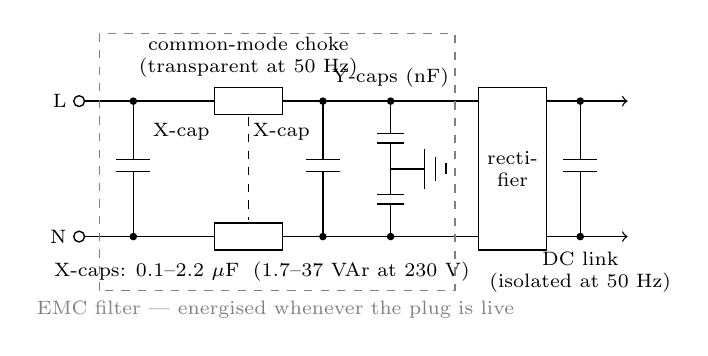
\begin{tikzpicture}[x=0.86mm, y=0.86mm, line width=0.5pt, font=\scriptsize]
% mains terminals and rails
\draw[fill=white] (2,20) circle (0.8) node[left=1pt] {L};
\draw[fill=white] (2,0) circle (0.8) node[left=1pt] {N};
\draw (2.8,20) -- (22,20);
\draw (2.8,0) -- (22,0);
% X1 capacitor
\draw (10,20) -- (10,11.4);
\draw (7.5,11.4) -- (12.5,11.4);
\draw (7.5,9.6) -- (12.5,9.6);
\draw (10,9.6) -- (10,0);
\filldraw (10,20) circle (0.45); \filldraw (10,0) circle (0.45);
\node[right=2pt] at (10.6,15.5) {X-cap};
% common-mode choke
\draw (22,18) rectangle (32,22);
\draw (22,-2) rectangle (32,2);
\draw[dashed] (27,17.6) -- (27,2.4);
\node[align=center] at (27,26.5) {common-mode choke\\(transparent at 50~Hz)};
\draw (32,20) -- (58,20);
\draw (32,0) -- (58,0);
% X2 capacitor
\draw (38,20) -- (38,11.4);
\draw (35.5,11.4) -- (40.5,11.4);
\draw (35.5,9.6) -- (40.5,9.6);
\draw (38,9.6) -- (38,0);
\filldraw (38,20) circle (0.45); \filldraw (38,0) circle (0.45);
\node[left=2pt, fill=white, inner sep=1pt] at (37.4,15.5) {X-cap};
\node[align=center, fill=white, inner sep=1pt] at (29,-5.2) {X-caps: $0.1$--$2.2~\mu$F\; ($1.7$--$37$~VAr at 230~V)};
% Y capacitors to earth
\draw (48,20) -- (48,15.2);
\draw (46,15.2) -- (50,15.2);
\draw (46,13.8) -- (50,13.8);
\draw (48,13.8) -- (48,10);
\draw (48,0) -- (48,4.8);
\draw (46,4.8) -- (50,4.8);
\draw (46,6.2) -- (50,6.2);
\draw (48,6.2) -- (48,10);
\filldraw (48,20) circle (0.45); \filldraw (48,0) circle (0.45);
\draw (48,10) -- (53,10);
\draw (53,13) -- (53,7);
\draw (54.6,11.8) -- (54.6,8.2);
\draw (56.2,10.8) -- (56.2,9.2);
\node at (48,23.5) {Y-caps (nF)};
% filter boundary
\draw[dashed, gray] (5,-8) rectangle (57.5,30);
\node[gray] at (31,-10.8) {EMC filter --- energised whenever the plug is live};
% rectifier and DC link
\draw (58,20) -- (61,20); \draw (58,0) -- (61,0);
\draw (61,-2) rectangle (71,22);
\node[align=center] at (66,10) {recti-\\fier};
\draw (71,20) -- (80,20); \draw (71,0) -- (80,0);
\draw (76,20) -- (76,11.4);
\draw (73.5,11.4) -- (78.5,11.4);
\draw (73.5,9.6) -- (78.5,9.6);
\draw (76,9.6) -- (76,0);
\filldraw (76,20) circle (0.45); \filldraw (76,0) circle (0.45);
\node[align=center] at (76,-5.2) {DC link\\(isolated at 50~Hz)};
\draw[->] (80,20) -- (83,20);
\draw[->] (80,0) -- (83,0);
\end{tikzpicture}
\caption{The mains input stage of a switched-mode device. The EMC filter's
X-capacitance sits directly across line and neutral, ahead of the rectifier and
of any standby switching, and injects $\omega C V^2$ of leading reactive power
whenever the plug is live; the
Y-capacitors are nanofarad-scale, and the large DC-link capacitor is isolated
from the fundamental behind the rectifier. Component values are datasheet-grade
typical ranges (Section~V-B); on North America's 120~V, 60~Hz mains the same
0.1--2.2~$\mu$F range injects 0.5--12~VAr.}
\label{fig:emifilter}
\end{figure}

\subsection{The aggregation asymmetry}
The two capacitor classes are governed on opposite principles, and the
contrast locates the regulatory gap precisely. The Y-capacitors'
earth-leakage current is treated as what it is---a current that accumulates.
It is budgeted per device: the touch-current allowance for ordinary
plug-connected equipment is 3.5~mA, and design practice dimensions the
Y-capacitance against that budget first~\cite{wurth_anp015}. It is budgeted
again per installation: the United Kingdom's wiring regulations, for
instance, require the accumulated protective-conductor current downstream of
a residual-current device to be not more than 30 per cent of its rated
residual operating current~\cite{bs7671}. Filter datasheets print the
consequence in their units, listing $C_x$ in microfarads beside $C_y$ in
nanofarads. The X-capacitance's reactive current accumulates across devices
in exactly the same way---the sum at a connection is tens of devices, at a
grid exit point whole fleets---but no analogous budget exists at any scale:
conducted-emission compliance is certified one device at a time against a
standardised artificial mains network (CISPR~16-1-2), the harmonic-current
standard is silent on fundamental reactive current (Section~I-A), and we are
not aware of any emission standard, wiring rule, or standards work item that
has considered the aggregate. Where the regime recognised an aggregating
current, it budgeted both the term and the sum; the standing reactive aggregate
has never been anyone's design variable.

\subsection{What does not count, and the grade of these values}
The three capacitor classes that dominate a device's capacitance budget but
contribute no standing fundamental-frequency injection---the DC-link
electrolytic, motor-run capacitors, and a rooftop inverter's converter-side
filter capacitors---and the one-way regulatory ratchet behind the accumulation
are set out in Section~V-B. The per-device values here are datasheet-grade,
not bench-measured; the aggregate rests on Section~V-B's labelled estimate;
and the decisive measurement is the low-voltage one identified in
Section~V-C.

\section*{Reproducibility}
Every number and figure in this paper is computed from public data (Electricity
Authority grid metering and Commerce Commission information disclosures) in an
accompanying set of analysis notebooks, which also document the path from the raw
public records. Both input sets are public and published under CC~BY~4.0---the grid
metering on the Electricity Authority's Electricity Market Information platform,
the network parameters in the Commerce Commission's information disclosures---and
the archived package carries the inputs themselves together with the retrieval
record and per-file checksums.

\section*{Acknowledgment}
The author thanks colleagues at the Electricity Authority and Transpower for
discussion of the reactive-power and voltage-management context, and the authors of
the Rhodes autonomous-system studies for sharing corrected source material.

The author used Anthropic's Claude models as a research assistant throughout this
work: literature searching, analysis and replication code, manuscript drafting and
editing, and verification passes over numbers and citations. The research questions,
analytical design, interpretation, and conclusions are the author's own. Every
printed number is reproduced from public data by the accompanying notebooks and
every citation was checked against its primary source; the author is responsible for
all content.

% Final-page column balance (standard IEEEtran practice). After the 7-Aug significance
% additions the references fill the final page naturally; the trigger is OFF. Re-enable
% \IEEEtriggeratref{N} only if a future edit strands a sliver page.
%\IEEEtriggeratref{30}
\bibliographystyle{IEEEtran}
\bibliography{refs}

\end{document}
